% =====================================================================
% Chapter 9: Sound radiation -- why the resonator lattice can make the
% plate louder
% Stage 7 follow-up, dispersion branch (Nov 2026)
% Requires: amsmath, amssymb, tikz (library arrows.meta)
% Include in the main file with  % =====================================================================
% Chapter 9: Sound radiation -- why the resonator lattice can make the
% plate louder
% Stage 7 follow-up, dispersion branch (Nov 2026)
% Requires: amsmath, amssymb, tikz (library arrows.meta)
% Include in the main file with  % =====================================================================
% Chapter 9: Sound radiation -- why the resonator lattice can make the
% plate louder
% Stage 7 follow-up, dispersion branch (Nov 2026)
% Requires: amsmath, amssymb, tikz (library arrows.meta)
% Include in the main file with  % =====================================================================
% Chapter 9: Sound radiation -- why the resonator lattice can make the
% plate louder
% Stage 7 follow-up, dispersion branch (Nov 2026)
% Requires: amsmath, amssymb, tikz (library arrows.meta)
% Include in the main file with  \include{chapter_09_radiation}
% =====================================================================

\chapter{Sound radiation: why the resonator lattice can make the plate louder}
\label{ch:radiation}

The finite $1 \times 1\,\mathrm{m}$ plate with $10 \times 10$ resonators on the
$0.1\,\mathrm{m}$ lattice ($f_r = 1.2\,\mathrm{kHz}$, $\mu = 0.25$) shows two
features in the insertion loss (IL) of the radiated power:
\begin{itemize}
  \item a peak of about $+13\,\mathrm{dB}$ inside the Bloch gap
        $1031$--$1195\,\mathrm{Hz}$ (Chapter~\ref{ch:complex_k}: evanescent
        waves);
  \item a dip of about $-14\,\mathrm{dB}$ at about $1260\,\mathrm{Hz}$, right at
        the flat resonator branch: \emph{with} resonators the plate radiates more
        than without.
\end{itemize}
This chapter explains the dip. The short version: the resonators do not make the
plate move more, they make it move in a shape that the air cannot short-circuit.

\begin{center}
\begin{tabular}{|l|p{0.5\textwidth}|l|}
\hline
Symbol & Meaning & Value at $1260\,\mathrm{Hz}$ \\
\hline
$c$, $\rho_0$ & speed of sound, density of air & $343\,\mathrm{m/s}$, $1.2\,\mathrm{kg/m^3}$ \\
$k_\mathrm{air} = \omega/c$ & acoustic wavenumber & $23.1\,\mathrm{rad/m}$ \\
$\lambda_\mathrm{air} = 2\pi/k_\mathrm{air}$ & acoustic wavelength & $27.2\,\mathrm{cm}$ \\
$D = E h^3/(12(1-\nu^2))$ & bending stiffness & $2404\,\mathrm{N\,m}$ \\
$k_b = (\omega^2 \rho h/D)^{1/4}$ & free bending wavenumber (Kirchhoff) & $31.8\,\mathrm{rad/m}$ \\
$\lambda_b = 2\pi/k_b$ & bending wavelength & $19.8\,\mathrm{cm}$ \\
$c_b = \omega/k_b$ & phase (trace) speed of the bending wave & $249\,\mathrm{m/s}$ \\
$k_x$ & wavenumber of a plate pattern along the surface & -- \\
$k_z$ & wavenumber of the air field normal to the plate & -- \\
$S$ & plate area & $1\,\mathrm{m^2}$ \\
$\langle v^2 \rangle$ & mean square normal velocity, averaged over the plate & -- \\
$W$ & radiated sound power & -- \\
$\sigma$ & radiation efficiency & -- \\
$f_c$ & critical (coincidence) frequency & $\approx 2.4\,\mathrm{kHz}$ \\
\hline
\end{tabular}
\end{center}

% ---------------------------------------------------------------------
\section{Radiation efficiency}

The radiated power is written as
\begin{equation}
  W = \rho_0 c\, S\, \langle v^2 \rangle\, \sigma .
  \label{eq:radiation_efficiency}
\end{equation}
$\rho_0 c S \langle v^2 \rangle$ is the power a rigid piston of the same area and
the same mean square velocity would radiate at high frequency. $\sigma$ says how
much of that the actual vibration pattern achieves: $\sigma \approx 1$ for a
piston-like pattern, $\sigma \ll 1$ for a pattern that ``wastes'' its motion.

Since the IL compares the radiated power of the bare plate with that of the plate
with resonators, Eq.~\eqref{eq:radiation_efficiency} splits it into two parts:
\begin{equation}
  \mathrm{IL} = 10\log_{10}\frac{W_\mathrm{bare}}{W_\mathrm{res}}
  = \underbrace{10\log_{10}\frac{\langle v^2\rangle_\mathrm{bare}}{\langle v^2\rangle_\mathrm{res}}}_{\text{velocity term}}
  + \underbrace{10\log_{10}\frac{\sigma_\mathrm{bare}}{\sigma_\mathrm{res}}}_{\text{efficiency term}} .
  \label{eq:il_split}
\end{equation}
The resonators can make the velocity term positive (less motion) and still produce
a negative IL if they raise $\sigma$ enough. This is what happens at the flat branch.

% ---------------------------------------------------------------------
\section{Subsonic and supersonic patterns}

\subsection{Trace matching}
Let the plate vibrate with a pattern $v(x) = \hat v\, e^{i k_x x}$ along its surface
(time factor $e^{i\omega t}$). At the surface the air must move with the plate, so
the air field has the same $k_x$. In air every field obeys the wave equation,
which for a plane-wave component $e^{i(k_x x + k_z z)}$ means
\begin{equation}
  k_x^2 + k_z^2 = k_\mathrm{air}^2
  \quad\Longrightarrow\quad
  k_z = \sqrt{k_\mathrm{air}^2 - k_x^2} .
\end{equation}
Two cases:
\begin{itemize}
  \item $k_x < k_\mathrm{air}$: $k_z$ is real, a plane wave leaves the plate at the
        angle $\alpha$ from the normal with $\sin\alpha = k_x/k_\mathrm{air}$. Power
        is carried away.
  \item $k_x > k_\mathrm{air}$: $k_z = \pm i\sqrt{k_x^2 - k_\mathrm{air}^2}$ is
        imaginary, the pressure decays like
        $e^{-z\sqrt{k_x^2 - k_\mathrm{air}^2}}$ away from the plate. This is a
        \emph{near field}; it carries no power.
\end{itemize}

\subsection{Why ``supersonic'' means \emph{small} $k$}
The names refer to the \emph{phase speed} of the pattern along the plate,
$c_\mathrm{trace} = \omega/k_x$, not to the material velocity (which is always tiny).
At fixed $\omega$ a larger wavenumber means a shorter wavelength and a slower
pattern:
\begin{equation}
  k_x < k_\mathrm{air} \;\Longleftrightarrow\; \frac{\omega}{k_x} > c
  \quad\text{(supersonic)},
  \qquad
  k_x > k_\mathrm{air} \;\Longleftrightarrow\; \frac{\omega}{k_x} < c
  \quad\text{(subsonic)} .
\end{equation}
For the bare plate at $1260\,\mathrm{Hz}$, $k_b = 31.8 > 23.1 = k_\mathrm{air}$:
the free bending wave is subsonic ($c_b = 249\,\mathrm{m/s} < 343\,\mathrm{m/s}$).
Its pressure decays with the length
$1/\sqrt{31.8^2 - 23.1^2}\,\mathrm{m} = 1/21.9\,\mathrm{m} \approx 4.6\,\mathrm{cm}$.

\subsection{The critical frequency}
Bending waves are dispersive: $f = \frac{1}{2\pi}\sqrt{D/(\rho h)}\, k_b^2$, so
$k_b \propto \sqrt{f}$, while $k_\mathrm{air} \propto f$. The air line overtakes the
bending curve at the critical frequency
\begin{equation}
  f_c = \frac{c^2}{2\pi}\sqrt{\frac{\rho h}{D}} \approx 2.4\,\mathrm{kHz}
  \quad (5\,\mathrm{mm} \text{ steel; RM gives about } 2.45\,\mathrm{kHz}).
\end{equation}
Below $f_c$ free bending waves are subsonic, above it supersonic.
Figure~\ref{fig:radiation_dispersion} shows both curves.

\begin{figure}[htbp]
\centering
\begin{tikzpicture}[x=0.11cm, y=0.0019cm, >={Stealth}]
  % radiation cone: k < k_air(f), i.e. left of the air line
  \fill[gray!18] (0,0) -- (54.9,3000) -- (0,3000) -- cycle;
  \node[align=left, font=\footnotesize] at (11,2550) {radiation cone\\ $k < k_\mathrm{air}$\\ (supersonic)};
  % axes
  \draw[->] (0,0) -- (57,0) node[below left] {$k$ (rad/m)};
  \draw[->] (0,0) -- (0,3250) node[above] {$f$ (Hz)};
  \foreach \kk in {10,20,30,40,50} \draw (\kk,0) -- (\kk,-60) node[below, font=\scriptsize] {\kk};
  \foreach \ff in {1000,2000,3000} \draw (0,\ff) -- (-1,\ff) node[left, font=\scriptsize] {\ff};
  % air line f = c k / (2 pi) = 54.6 k
  \draw[thick, dashed] (0,0) -- (54.9,3000) node[above, font=\footnotesize] {air: $f = c k/2\pi$};
  % bare bending curve f = 1.245 k^2
  \draw[thick] plot[domain=0:49, samples=60] (\x, {1.245*\x*\x});
  \node[font=\footnotesize, right] at (47,2500) {bare plate};
  % flat resonator branch (schematic)
  \draw[very thick, gray] (0,1270) -- (44.4,1270);
  \node[font=\footnotesize, gray, right] at (44.4,1270) {flat resonator branch};
  % 1260 Hz markers
  \draw[dotted] (0,1260) -- (31.8,1260);
  \draw[dotted] (23.1,0) -- (23.1,1260);
  \draw[dotted] (31.8,0) -- (31.8,1260);
  \fill (23.1,1260) circle (1.2pt);
  \fill (31.8,1260) circle (1.2pt);
  \node[font=\scriptsize, below] at (21.5,500) {$k_\mathrm{air}$};
  \node[font=\scriptsize, below] at (34,500) {$k_b$};
  % critical frequency
  \fill (43.9,2396) circle (1.5pt) node[right, font=\footnotesize] {$f_c$};
\end{tikzpicture}
\caption{Bending curve (Kirchhoff, $5\,\mathrm{mm}$ steel) and air line. Shaded:
patterns with $k < k_\mathrm{air}$, which radiate. At $1260\,\mathrm{Hz}$ the bare
plate only has $k_b = 31.8\,\mathrm{rad/m}$, outside the cone. The flat resonator
branch (schematic, gray) offers states at about $1270\,\mathrm{Hz}$ for every
$\mathbf{k}$, including small $k$ inside the cone.}
\label{fig:radiation_dispersion}
\end{figure}

% ---------------------------------------------------------------------
\section{The acoustic short circuit}

\subsection{The time argument}
A crest of the plate pushes air out, the neighboring trough sucks air in. The
pushed air can flow sideways into the trough if it gets there before the plate
reverses, i.e.\ within half a period $T/2$. Disturbances in air travel at $c$, so
in that time they cover
\begin{equation}
  c\,\frac{T}{2} = \frac{\lambda_\mathrm{air}}{2} .
\end{equation}
The trough is $\lambda_b/2$ away. The short circuit works if
\begin{equation}
  \frac{\lambda_b}{2} < \frac{\lambda_\mathrm{air}}{2}
  \;\Longleftrightarrow\; \lambda_b < \lambda_\mathrm{air}
  \;\Longleftrightarrow\; k_b > k_\mathrm{air}
  \;\Longleftrightarrow\; \text{subsonic} .
\end{equation}
The time argument is the trace-matching condition in words. At $1260\,\mathrm{Hz}$
the trough is $9.9\,\mathrm{cm}$ away and sound covers $13.6\,\mathrm{cm}$ in half a
period: the air gets there in time (Figure~\ref{fig:short_circuit}).

\begin{figure}[htbp]
\centering
\begin{tikzpicture}[x=1cm, y=1cm, >={Stealth}]
  % plate: half wavelength = 1 unit = 9.9 cm
  \draw[thick] plot[domain=0:8, samples=200] (\x, {0.3*sin(\x*180)});
  \foreach \xx in {0.5,2.5,4.5,6.5} \node[font=\footnotesize] at (\xx,-0.2) {$+$};
  \foreach \xx in {1.5,3.5,5.5,7.5} \node[font=\footnotesize] at (\xx,0.2) {$-$};
  % sideways air flow from crests into troughs
  \foreach \xx in {0.5,2.5,4.5,6.5} {
    \draw[->, gray] (\xx+0.1,0.55) -- (\xx+0.9,0.55);
    \draw[->, gray] (\xx-0.1,0.55) -- (\xx-0.9,0.55);
  }
  % distances
  \draw[|<->|] (0.5,-0.75) -- (1.5,-0.75) node[midway, below, font=\footnotesize] {$\lambda_b/2 = 9.9\,\mathrm{cm}$};
  \draw[|<->|] (4.5,-0.75) -- (5.87,-0.75) node[midway, below, font=\footnotesize] {$\lambda_\mathrm{air}/2 = 13.6\,\mathrm{cm}$};
  \node[font=\footnotesize, gray] at (4,1.0) {air sloshes sideways: short circuit, almost nothing leaves};
\end{tikzpicture}
\caption{Bare plate at $1260\,\mathrm{Hz}$ (side view). In half a period, sound
travels farther ($13.6\,\mathrm{cm}$) than the distance from crest to trough
($9.9\,\mathrm{cm}$): the air flows sideways instead of outward.}
\label{fig:short_circuit}
\end{figure}

\subsection{The same in the near field}
Figure~\ref{fig:near_far} shows what the trace-matching result means for the
pressure. On the left, the subsonic ripple: the pressure pattern above the plate
dies out within a few centimeters. On the right, a supersonic pattern: wavefronts
leave the plate at the angle $\alpha$.

\begin{figure}[htbp]
\centering
\begin{tikzpicture}[x=1cm, y=1cm, >={Stealth}]
  % left: subsonic, 1 unit = 9.9 cm, decay length 0.46 units
  \begin{scope}
    \draw[thick] plot[domain=0:4, samples=120] (\x, {0.3*sin(\x*180)});
    \foreach \zz in {0.4,0.8,1.2,1.6} {
      \draw[gray] plot[domain=0:4, samples=120] (\x, {\zz + 0.3*exp(-\zz/0.46)*sin(\x*180)});
    }
    \node[font=\footnotesize, align=center] at (2,2.3) {subsonic ($k_x = 31.8\,\mathrm{rad/m}$)\\ pressure dies out within $\sim 5\,\mathrm{cm}$};
  \end{scope}
  % right: supersonic, long wavelength, slanted wavefronts
  \begin{scope}[xshift=5.5cm]
    \draw[thick] plot[domain=0:4, samples=120] (\x, {0.3*sin(\x*45)});
    \foreach \s in {0,0.6,1.2,1.8,2.4} {
      \draw[gray] (\s,0.35) -- (\s+1.2,1.85);
    }
    \draw[->] (2.2,0.6) -- (2.95,1.2) node[right, font=\footnotesize] {sound};
    \node[font=\footnotesize, align=center] at (2,2.3) {supersonic ($k_x < k_\mathrm{air}$)\\ wavefronts leave at $\sin\alpha = k_x/k_\mathrm{air}$};
  \end{scope}
\end{tikzpicture}
\caption{Left: lines of equal height show the pressure amplitude above a subsonic
ripple, decaying like $e^{-z/4.6\,\mathrm{cm}}$. Right: a long-wavelength
(supersonic) pattern sends plane waves into the air.}
\label{fig:near_far}
\end{figure}

\subsection{Why the bare finite plate radiates at all}
On a finite plate, every $+$ region of a subsonic mode has a $-$ neighbor that
cancels it, except where the pattern ends. The uncanceled strips along the edges
and the uncanceled corner cells radiate (Figure~\ref{fig:edge_radiation}). Their
area is small compared with the plate, so $\sigma \ll 1$. For the bare modes near
$1260\,\mathrm{Hz}$ the modal analysis (open check (b)) gave
$\sigma = 0.003$--$0.014$.

\begin{figure}[htbp]
\centering
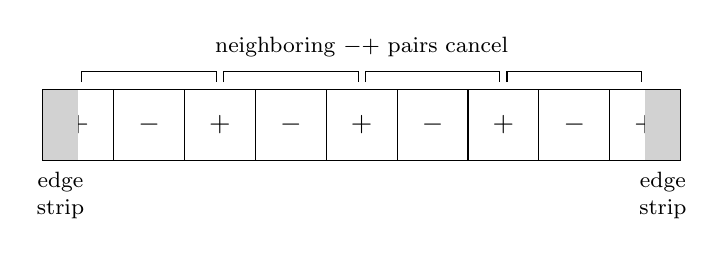
\begin{tikzpicture}[x=0.9cm, y=0.9cm]
  \foreach \i in {0,...,8} {
    \draw (\i,0) rectangle (\i+1,1);
    \ifodd\i \node at (\i+0.5,0.5) {$-$}; \else \node at (\i+0.5,0.5) {$+$}; \fi
  }
  \fill[gray!35] (0,0) rectangle (0.5,1);
  \fill[gray!35] (8.5,0) rectangle (9,1);
  \draw (0,0) rectangle (9,1);
  \foreach \i in {0.5,2.5,4.5,6.5} {
    \draw (\i+0.05,1.1) -- (\i+0.05,1.25) -- (\i+1.95,1.25) -- (\i+1.95,1.1);
  }
  \node[font=\footnotesize] at (4.5,1.6) {neighboring $-{}+$ pairs cancel};
  \node[font=\footnotesize, align=center] at (0.25,-0.5) {edge\\strip};
  \node[font=\footnotesize, align=center] at (8.75,-0.5) {edge\\strip};
\end{tikzpicture}
\caption{One row of half-wavelength regions of a subsonic mode. Pairs cancel; only
the unpaired strips at the edges (gray, and in 2D the corners) are left to radiate.}
\label{fig:edge_radiation}
\end{figure}

% ---------------------------------------------------------------------
\section{What the resonators change}

\subsection{They add small-$k$ states at $1270\,\mathrm{Hz}$}
At $1260\,\mathrm{Hz}$ the bare plate has no choice: every free motion has
$k = k_b = 31.8\,\mathrm{rad/m}$. The flat resonator branch
(Chapter~\ref{ch:local_resonance}) provides modes at about $1270\,\mathrm{Hz}$
for \emph{every} $\mathbf{k}$ in the Brillouin zone, including small $|\mathbf{k}|$
inside the radiation cone (Figure~\ref{fig:radiation_dispersion}). The resonators
do not smooth out the bare mode; they create a kind of mode that the bare plate
cannot have at this frequency.

\subsection{What a flat-branch mode looks like}
By Bloch's theorem (Chapter~\ref{ch:bloch}) a mode on the flat branch is
\begin{equation}
  w(\mathbf{x}) = e^{i\mathbf{k}\cdot\mathbf{x}}\; p(\mathbf{x}),
  \qquad p \text{ cell-periodic},
\end{equation}
a slowly varying envelope $e^{i\mathbf{k}\cdot\mathbf{x}}$ times the same cell
pattern $p$ in every cell.

\paragraph{The cell pattern near $\Gamma$.}
In the in-phase mode the resonator mass bounces on its spring and the plate cell
recoils. With the resonator amplitude $u$ and the mean plate displacement
$\bar w$ of the cell, momentum balance per cell (no external force) gives
\begin{equation}
  m\,u + \rho h A\, \bar w = 0
  \quad\Longrightarrow\quad
  \bar w = -\mu\, u = -0.25\,u .
\end{equation}
The whole cell moves opposite to the resonator with a quarter of its amplitude. On
top of that sits a local dimple under the attachment point, where the spring force
bends the plate (Figure~\ref{fig:cell_pattern}). The dimple is what lowers the
frequency from $f_r\sqrt{1+\mu} = 1342\,\mathrm{Hz}$ (rigid cell) to the FE value
of $1273\,\mathrm{Hz}$ (Chapter~\ref{ch:gap_position}).

\begin{figure}[htbp]
\centering
\begin{tikzpicture}[x=1cm, y=1cm, >={Stealth}]
  % undeformed plate (reference)
  \draw[gray, dashed] (0,0) -- (5,0);
  \node[gray, font=\footnotesize, left] at (0,0) {rest};
  % deformed plate: shifted down by 0.25 with a dimple at x = 2.5
  \draw[thick] plot[domain=0:5, samples=150] (\x, {-0.35 - 0.25*exp(-((\x-2.5)^2)/0.15)});
  % spring
  \draw (2.5,-0.6) -- (2.5,-0.45) -- (2.35,-0.35) -- (2.65,-0.15) -- (2.35,0.05)
        -- (2.65,0.25) -- (2.35,0.45) -- (2.5,0.55) -- (2.5,0.7);
  % mass
  \draw[fill=gray!30] (2.1,0.7) rectangle (2.9,1.2);
  \node[font=\footnotesize] at (2.5,0.95) {$m$};
  \draw[->, thick] (3.2,0.95) -- (3.2,1.55) node[right, font=\footnotesize] {$u$};
  \draw[->, thick] (4.4,-0.05) -- (4.4,-0.35) node[right, font=\footnotesize] {$\bar w = -\mu u$};
  \node[font=\footnotesize] at (1.0,-0.85) {one cell ($10\,\mathrm{cm}$)};
  \node[font=\footnotesize] at (3.6,-0.85) {dimple};
\end{tikzpicture}
\caption{Cell pattern of the in-phase mode near $\Gamma$ (exaggerated): the cell
moves down as a whole while the resonator moves up, with a local dimple at the
attachment point.}
\label{fig:cell_pattern}
\end{figure}

\paragraph{The finite plate.}
The 40 modes of the finite plate between $1246$ and $1282\,\mathrm{Hz}$ are
66--78\,\% resonator motion. Each repeats the cell pattern under a smooth envelope
that varies over the whole plate, like the low-order modes of a $10 \times 10$ grid
of masses. Split the plate motion into two parts (Figure~\ref{fig:smooth_ripple}):
\begin{itemize}
  \item the \textbf{smooth part}: cell means $\bar w$ times the envelope;
  \item the \textbf{ripple}: the dimples, repeated in every cell.
\end{itemize}

\begin{figure}[htbp]
\centering
\begin{tikzpicture}[x=1cm, y=1cm, >={Stealth}]
  % resonator amplitudes following the envelope sin(pi x / 10), 10 cells over 10 units
  \begin{scope}[yshift=3.6cm]
    \foreach \i in {0,...,9} {
      \pgfmathsetmacro{\amp}{0.7*sin((\i+0.5)*18)}
      \draw[->, thick] (\i+0.5,0) -- (\i+0.5,\amp);
    }
    \draw[gray] (0,0) -- (10,0);
    \node[font=\footnotesize, left] at (0,0.3) {resonators};
  \end{scope}
  % smooth part
  \begin{scope}[yshift=2.2cm]
    \draw[gray, dashed] (0,0) -- (10,0);
    \draw[thick] plot[domain=0:10, samples=100] (\x, {-0.5*sin(\x*18)});
    \node[font=\footnotesize, left, align=right] at (0,0) {smooth part\\ $k \approx \pi/L$};
  \end{scope}
  % ripple
  \begin{scope}[yshift=1.0cm]
    \draw[gray, dashed] (0,0) -- (10,0);
    \draw[thick] plot[domain=0:10, samples=400] (\x, {-0.2*sin(\x*18)*exp(-((\x-floor(\x)-0.5)^2)/0.02)});
    \node[font=\footnotesize, left, align=right] at (0,0) {ripple\\ $k \ge 2\pi/a$};
  \end{scope}
  % total
  \begin{scope}[yshift=-0.4cm]
    \draw[gray, dashed] (0,0) -- (10,0);
    \draw[thick] plot[domain=0:10, samples=400] (\x, {-0.5*sin(\x*18) - 0.2*sin(\x*18)*exp(-((\x-floor(\x)-0.5)^2)/0.02)});
    \node[font=\footnotesize, left] at (0,0) {plate};
  \end{scope}
  \draw[|<->|] (0,-1.3) -- (10,-1.3) node[midway, below, font=\footnotesize] {$L = 1\,\mathrm{m}$, 10 cells};
\end{tikzpicture}
\caption{A low-order cluster mode (side view, schematic). Top: resonator
amplitudes follow a smooth envelope. Below: the plate motion is a smooth part
(cell means, opposite to the resonators) plus a ripple of dimples, one per cell.}
\label{fig:smooth_ripple}
\end{figure}

\subsection{Which part radiates}
\begin{center}
\begin{tabular}{|l|p{0.28\textwidth}|p{0.18\textwidth}|p{0.27\textwidth}|}
\hline
Part & Wavenumbers & vs.\ $k_\mathrm{air} = 23.1\,\mathrm{rad/m}$ & Radiates? \\
\hline
smooth part & envelope: $m\pi/L = 3.1, 6.3, 9.4, \dots\,\mathrm{rad/m}$ & inside the cone for low orders & yes: $+$ and $-$ regions tens of cm apart \\
ripple & $\ge 2\pi/a = 62.8\,\mathrm{rad/m}$ & far outside & no: decay length $1/\sqrt{62.8^2 - 23.1^2}\,\mathrm{m} = 1.7\,\mathrm{cm}$ \\
\hline
\end{tabular}
\end{center}
In the extreme case of a uniform envelope ($\mathbf{k} = 0$), all cell means move in
phase and the plate acts as a piston. A rough estimate (not computed): envelope
orders up to $m \approx 7$ satisfy $m\pi/L < 23.1\,\mathrm{rad/m}$ on the
$1\,\mathrm{m}$ plate, which fits the observation that most, but not all, cluster
modes radiate strongly.

\paragraph{Why the plate simply follows the resonators.}
For a force pattern with wavenumber $k$ the plate responds (Kirchhoff, undamped) with
\begin{equation}
  \hat w(k) = \frac{\hat F(k)}{D k^4 - \rho h\,\omega^2}
  \;\overset{k \ll k_b}{\approx}\; -\frac{\hat F(k)}{\rho h\,\omega^2} .
\end{equation}
At small $k$ the bending stiffness $D k^4$ is negligible; the plate acts like a mass
and moves with whatever smooth pattern the resonators impose. The plate goes where
the resonators push it, and they push smoothly.

\subsection{The numbers}
From the modal analysis of the finite plate (open check (b),
\texttt{check\_finite\_plate\_modes.py}):
\begin{center}
\begin{tabular}{|l|l|}
\hline
Modes & Radiation efficiency $\sigma$ \\
\hline
bare plate, near $1260\,\mathrm{Hz}$ & $0.003$--$0.014$ \\
cluster $1246$--$1282\,\mathrm{Hz}$, $2\times 2$ shear rule & $0.35$--$0.90$ \\
cluster, full $3\times 3$ shear rule & $0.54$--$0.80$ \\
\hline
\end{tabular}
\end{center}
Per unit velocity the cluster modes radiate about $20\,\mathrm{dB}$ more than the bare
modes. In Eq.~\eqref{eq:il_split} the efficiency term is then about
$10\log_{10}(0.01/0.5) \approx -17\,\mathrm{dB}$, which the velocity term cannot
compensate: the IL dips to about $-14\,\mathrm{dB}$. (Rough: in the forced response
several modes overlap, so the modal $\sigma$ values only bracket the effective one.)
With the full $3\times 3$ shear rule, now used throughout, the dip is
$-13.9\,\mathrm{dB}$ at $1267\,\mathrm{Hz}$.

\paragraph{Inside a gap: the $600\,\mathrm{Hz}$ tuning.} The same mechanism can reach into
a gap. With $f_r = 600\,\mathrm{Hz}$ ($\tau = 0.5$, Bloch gap $578$--$662\,\mathrm{Hz}$) the
IL turns negative from $633\,\mathrm{Hz}$ on, about $65\,\%$ into the gap. Averaged over
$628$--$662\,\mathrm{Hz}$: IL $-7.4\,\mathrm{dB}$ = velocity term $+7.8\,\mathrm{dB}$ +
efficiency term $-15.2\,\mathrm{dB}$. The plate does move less, as the gap requires, but the
remaining motion radiates far better. At this tuning the upper gap edge \emph{is} the
resonator band at $\Gamma$ (small $k$, supersonic), and the bare plate, four times below
$f_c$, radiates very poorly. At $1200\,\mathrm{Hz}$ the upper edge is the sin pattern at
$X$, which is subsonic ($31.4$ against $21.9\,\mathrm{rad/m}$), and the efficiency term
inside the gap stays near $-3\,\mathrm{dB}$.

% ---------------------------------------------------------------------
\section{Summary}
\begin{enumerate}
  \item Below $f_c \approx 2.4\,\mathrm{kHz}$ free bending waves are subsonic
        ($k_b > k_\mathrm{air}$); the air short-circuits between neighboring crests
        and troughs, and only edges and corners radiate ($\sigma \sim 0.01$).
  \item The flat resonator branch provides modes at about $1270\,\mathrm{Hz}$ for all
        $\mathbf{k}$, including small $\mathbf{k}$ inside the radiation cone.
  \item In these modes the plate moves as cell means (opposite to the resonators,
        $\bar w = -\mu u$) under a smooth envelope, plus a ripple of dimples. The
        smooth part is supersonic and radiates ($\sigma \sim 0.5$); the ripple does not.
  \item The plate does not move more, it moves in a shape the air cannot short-circuit:
        the efficiency term of the IL is about $-17\,\mathrm{dB}$, giving the
        $-14\,\mathrm{dB}$ dip.
\end{enumerate}

% ---------------------------------------------------------------------
\section{Check questions with answers}

\paragraph{Question 1.} \emph{Would the bare plate radiate better at
$2000\,\mathrm{Hz}$ than at $1260\,\mathrm{Hz}$? Use the wavenumbers.}

\emph{Answer.} Yes. $k_b \propto \sqrt{f}$: $k_b(2000) = 31.8\sqrt{2000/1260} =
40.1\,\mathrm{rad/m}$, while $k_\mathrm{air}(2000) = 2\pi\cdot 2000/343 =
36.6\,\mathrm{rad/m}$. Still subsonic, but much closer to coincidence: the decay
length grows from $4.6\,\mathrm{cm}$ to $1/\sqrt{40.1^2 - 36.6^2}\,\mathrm{m} \approx
6.1\,\mathrm{cm}$, and crest and trough are $7.8\,\mathrm{cm}$ apart against
$8.6\,\mathrm{cm}$ covered by sound in half a period. The short circuit becomes
incomplete; $\sigma$ rises towards its maximum near $f_c$.

\paragraph{Question 2.} \emph{The resonators push hardest right at the attachment
points, where the dimples are. Why does that motion not radiate?}

\emph{Answer.} The dimples repeat with the lattice period, so their wavenumbers are at
least $2\pi/a = 62.8\,\mathrm{rad/m}$, almost three times $k_\mathrm{air}$. Their
pressure decays with a length of $1.7\,\mathrm{cm}$: each dimple is short-circuited by
the surrounding plate, which moves the other way. Only the cell means, collected under
a smooth envelope, reach the far field.

\paragraph{Question 3.} \emph{Resonators tuned to $3\,\mathrm{kHz}$, above $f_c$: would
the same IL dip appear at their flat branch?}

\emph{Answer (expectation, not computed).} Much weaker. Above $f_c$ the bare plate's
free waves are already supersonic and radiate with $\sigma \approx 1$. The flat branch
cannot raise $\sigma$ much further, so the efficiency term of
Eq.~\eqref{eq:il_split} is small, and the IL is governed by the velocity term. The dip
is a below-coincidence effect.

% =====================================================================

\chapter{Sound radiation: why the resonator lattice can make the plate louder}
\label{ch:radiation}

The finite $1 \times 1\,\mathrm{m}$ plate with $10 \times 10$ resonators on the
$0.1\,\mathrm{m}$ lattice ($f_r = 1.2\,\mathrm{kHz}$, $\mu = 0.25$) shows two
features in the insertion loss (IL) of the radiated power:
\begin{itemize}
  \item a peak of about $+13\,\mathrm{dB}$ inside the Bloch gap
        $1031$--$1195\,\mathrm{Hz}$ (Chapter~\ref{ch:complex_k}: evanescent
        waves);
  \item a dip of about $-14\,\mathrm{dB}$ at about $1260\,\mathrm{Hz}$, right at
        the flat resonator branch: \emph{with} resonators the plate radiates more
        than without.
\end{itemize}
This chapter explains the dip. The short version: the resonators do not make the
plate move more, they make it move in a shape that the air cannot short-circuit.

\begin{center}
\begin{tabular}{|l|p{0.5\textwidth}|l|}
\hline
Symbol & Meaning & Value at $1260\,\mathrm{Hz}$ \\
\hline
$c$, $\rho_0$ & speed of sound, density of air & $343\,\mathrm{m/s}$, $1.2\,\mathrm{kg/m^3}$ \\
$k_\mathrm{air} = \omega/c$ & acoustic wavenumber & $23.1\,\mathrm{rad/m}$ \\
$\lambda_\mathrm{air} = 2\pi/k_\mathrm{air}$ & acoustic wavelength & $27.2\,\mathrm{cm}$ \\
$D = E h^3/(12(1-\nu^2))$ & bending stiffness & $2404\,\mathrm{N\,m}$ \\
$k_b = (\omega^2 \rho h/D)^{1/4}$ & free bending wavenumber (Kirchhoff) & $31.8\,\mathrm{rad/m}$ \\
$\lambda_b = 2\pi/k_b$ & bending wavelength & $19.8\,\mathrm{cm}$ \\
$c_b = \omega/k_b$ & phase (trace) speed of the bending wave & $249\,\mathrm{m/s}$ \\
$k_x$ & wavenumber of a plate pattern along the surface & -- \\
$k_z$ & wavenumber of the air field normal to the plate & -- \\
$S$ & plate area & $1\,\mathrm{m^2}$ \\
$\langle v^2 \rangle$ & mean square normal velocity, averaged over the plate & -- \\
$W$ & radiated sound power & -- \\
$\sigma$ & radiation efficiency & -- \\
$f_c$ & critical (coincidence) frequency & $\approx 2.4\,\mathrm{kHz}$ \\
\hline
\end{tabular}
\end{center}

% ---------------------------------------------------------------------
\section{Radiation efficiency}

The radiated power is written as
\begin{equation}
  W = \rho_0 c\, S\, \langle v^2 \rangle\, \sigma .
  \label{eq:radiation_efficiency}
\end{equation}
$\rho_0 c S \langle v^2 \rangle$ is the power a rigid piston of the same area and
the same mean square velocity would radiate at high frequency. $\sigma$ says how
much of that the actual vibration pattern achieves: $\sigma \approx 1$ for a
piston-like pattern, $\sigma \ll 1$ for a pattern that ``wastes'' its motion.

Since the IL compares the radiated power of the bare plate with that of the plate
with resonators, Eq.~\eqref{eq:radiation_efficiency} splits it into two parts:
\begin{equation}
  \mathrm{IL} = 10\log_{10}\frac{W_\mathrm{bare}}{W_\mathrm{res}}
  = \underbrace{10\log_{10}\frac{\langle v^2\rangle_\mathrm{bare}}{\langle v^2\rangle_\mathrm{res}}}_{\text{velocity term}}
  + \underbrace{10\log_{10}\frac{\sigma_\mathrm{bare}}{\sigma_\mathrm{res}}}_{\text{efficiency term}} .
  \label{eq:il_split}
\end{equation}
The resonators can make the velocity term positive (less motion) and still produce
a negative IL if they raise $\sigma$ enough. This is what happens at the flat branch.

% ---------------------------------------------------------------------
\section{Subsonic and supersonic patterns}

\subsection{Trace matching}
Let the plate vibrate with a pattern $v(x) = \hat v\, e^{i k_x x}$ along its surface
(time factor $e^{i\omega t}$). At the surface the air must move with the plate, so
the air field has the same $k_x$. In air every field obeys the wave equation,
which for a plane-wave component $e^{i(k_x x + k_z z)}$ means
\begin{equation}
  k_x^2 + k_z^2 = k_\mathrm{air}^2
  \quad\Longrightarrow\quad
  k_z = \sqrt{k_\mathrm{air}^2 - k_x^2} .
\end{equation}
Two cases:
\begin{itemize}
  \item $k_x < k_\mathrm{air}$: $k_z$ is real, a plane wave leaves the plate at the
        angle $\alpha$ from the normal with $\sin\alpha = k_x/k_\mathrm{air}$. Power
        is carried away.
  \item $k_x > k_\mathrm{air}$: $k_z = \pm i\sqrt{k_x^2 - k_\mathrm{air}^2}$ is
        imaginary, the pressure decays like
        $e^{-z\sqrt{k_x^2 - k_\mathrm{air}^2}}$ away from the plate. This is a
        \emph{near field}; it carries no power.
\end{itemize}

\subsection{Why ``supersonic'' means \emph{small} $k$}
The names refer to the \emph{phase speed} of the pattern along the plate,
$c_\mathrm{trace} = \omega/k_x$, not to the material velocity (which is always tiny).
At fixed $\omega$ a larger wavenumber means a shorter wavelength and a slower
pattern:
\begin{equation}
  k_x < k_\mathrm{air} \;\Longleftrightarrow\; \frac{\omega}{k_x} > c
  \quad\text{(supersonic)},
  \qquad
  k_x > k_\mathrm{air} \;\Longleftrightarrow\; \frac{\omega}{k_x} < c
  \quad\text{(subsonic)} .
\end{equation}
For the bare plate at $1260\,\mathrm{Hz}$, $k_b = 31.8 > 23.1 = k_\mathrm{air}$:
the free bending wave is subsonic ($c_b = 249\,\mathrm{m/s} < 343\,\mathrm{m/s}$).
Its pressure decays with the length
$1/\sqrt{31.8^2 - 23.1^2}\,\mathrm{m} = 1/21.9\,\mathrm{m} \approx 4.6\,\mathrm{cm}$.

\subsection{The critical frequency}
Bending waves are dispersive: $f = \frac{1}{2\pi}\sqrt{D/(\rho h)}\, k_b^2$, so
$k_b \propto \sqrt{f}$, while $k_\mathrm{air} \propto f$. The air line overtakes the
bending curve at the critical frequency
\begin{equation}
  f_c = \frac{c^2}{2\pi}\sqrt{\frac{\rho h}{D}} \approx 2.4\,\mathrm{kHz}
  \quad (5\,\mathrm{mm} \text{ steel; RM gives about } 2.45\,\mathrm{kHz}).
\end{equation}
Below $f_c$ free bending waves are subsonic, above it supersonic.
Figure~\ref{fig:radiation_dispersion} shows both curves.

\begin{figure}[htbp]
\centering
\begin{tikzpicture}[x=0.11cm, y=0.0019cm, >={Stealth}]
  % radiation cone: k < k_air(f), i.e. left of the air line
  \fill[gray!18] (0,0) -- (54.9,3000) -- (0,3000) -- cycle;
  \node[align=left, font=\footnotesize] at (11,2550) {radiation cone\\ $k < k_\mathrm{air}$\\ (supersonic)};
  % axes
  \draw[->] (0,0) -- (57,0) node[below left] {$k$ (rad/m)};
  \draw[->] (0,0) -- (0,3250) node[above] {$f$ (Hz)};
  \foreach \kk in {10,20,30,40,50} \draw (\kk,0) -- (\kk,-60) node[below, font=\scriptsize] {\kk};
  \foreach \ff in {1000,2000,3000} \draw (0,\ff) -- (-1,\ff) node[left, font=\scriptsize] {\ff};
  % air line f = c k / (2 pi) = 54.6 k
  \draw[thick, dashed] (0,0) -- (54.9,3000) node[above, font=\footnotesize] {air: $f = c k/2\pi$};
  % bare bending curve f = 1.245 k^2
  \draw[thick] plot[domain=0:49, samples=60] (\x, {1.245*\x*\x});
  \node[font=\footnotesize, right] at (47,2500) {bare plate};
  % flat resonator branch (schematic)
  \draw[very thick, gray] (0,1270) -- (44.4,1270);
  \node[font=\footnotesize, gray, right] at (44.4,1270) {flat resonator branch};
  % 1260 Hz markers
  \draw[dotted] (0,1260) -- (31.8,1260);
  \draw[dotted] (23.1,0) -- (23.1,1260);
  \draw[dotted] (31.8,0) -- (31.8,1260);
  \fill (23.1,1260) circle (1.2pt);
  \fill (31.8,1260) circle (1.2pt);
  \node[font=\scriptsize, below] at (21.5,500) {$k_\mathrm{air}$};
  \node[font=\scriptsize, below] at (34,500) {$k_b$};
  % critical frequency
  \fill (43.9,2396) circle (1.5pt) node[right, font=\footnotesize] {$f_c$};
\end{tikzpicture}
\caption{Bending curve (Kirchhoff, $5\,\mathrm{mm}$ steel) and air line. Shaded:
patterns with $k < k_\mathrm{air}$, which radiate. At $1260\,\mathrm{Hz}$ the bare
plate only has $k_b = 31.8\,\mathrm{rad/m}$, outside the cone. The flat resonator
branch (schematic, gray) offers states at about $1270\,\mathrm{Hz}$ for every
$\mathbf{k}$, including small $k$ inside the cone.}
\label{fig:radiation_dispersion}
\end{figure}

% ---------------------------------------------------------------------
\section{The acoustic short circuit}

\subsection{The time argument}
A crest of the plate pushes air out, the neighboring trough sucks air in. The
pushed air can flow sideways into the trough if it gets there before the plate
reverses, i.e.\ within half a period $T/2$. Disturbances in air travel at $c$, so
in that time they cover
\begin{equation}
  c\,\frac{T}{2} = \frac{\lambda_\mathrm{air}}{2} .
\end{equation}
The trough is $\lambda_b/2$ away. The short circuit works if
\begin{equation}
  \frac{\lambda_b}{2} < \frac{\lambda_\mathrm{air}}{2}
  \;\Longleftrightarrow\; \lambda_b < \lambda_\mathrm{air}
  \;\Longleftrightarrow\; k_b > k_\mathrm{air}
  \;\Longleftrightarrow\; \text{subsonic} .
\end{equation}
The time argument is the trace-matching condition in words. At $1260\,\mathrm{Hz}$
the trough is $9.9\,\mathrm{cm}$ away and sound covers $13.6\,\mathrm{cm}$ in half a
period: the air gets there in time (Figure~\ref{fig:short_circuit}).

\begin{figure}[htbp]
\centering
\begin{tikzpicture}[x=1cm, y=1cm, >={Stealth}]
  % plate: half wavelength = 1 unit = 9.9 cm
  \draw[thick] plot[domain=0:8, samples=200] (\x, {0.3*sin(\x*180)});
  \foreach \xx in {0.5,2.5,4.5,6.5} \node[font=\footnotesize] at (\xx,-0.2) {$+$};
  \foreach \xx in {1.5,3.5,5.5,7.5} \node[font=\footnotesize] at (\xx,0.2) {$-$};
  % sideways air flow from crests into troughs
  \foreach \xx in {0.5,2.5,4.5,6.5} {
    \draw[->, gray] (\xx+0.1,0.55) -- (\xx+0.9,0.55);
    \draw[->, gray] (\xx-0.1,0.55) -- (\xx-0.9,0.55);
  }
  % distances
  \draw[|<->|] (0.5,-0.75) -- (1.5,-0.75) node[midway, below, font=\footnotesize] {$\lambda_b/2 = 9.9\,\mathrm{cm}$};
  \draw[|<->|] (4.5,-0.75) -- (5.87,-0.75) node[midway, below, font=\footnotesize] {$\lambda_\mathrm{air}/2 = 13.6\,\mathrm{cm}$};
  \node[font=\footnotesize, gray] at (4,1.0) {air sloshes sideways: short circuit, almost nothing leaves};
\end{tikzpicture}
\caption{Bare plate at $1260\,\mathrm{Hz}$ (side view). In half a period, sound
travels farther ($13.6\,\mathrm{cm}$) than the distance from crest to trough
($9.9\,\mathrm{cm}$): the air flows sideways instead of outward.}
\label{fig:short_circuit}
\end{figure}

\subsection{The same in the near field}
Figure~\ref{fig:near_far} shows what the trace-matching result means for the
pressure. On the left, the subsonic ripple: the pressure pattern above the plate
dies out within a few centimeters. On the right, a supersonic pattern: wavefronts
leave the plate at the angle $\alpha$.

\begin{figure}[htbp]
\centering
\begin{tikzpicture}[x=1cm, y=1cm, >={Stealth}]
  % left: subsonic, 1 unit = 9.9 cm, decay length 0.46 units
  \begin{scope}
    \draw[thick] plot[domain=0:4, samples=120] (\x, {0.3*sin(\x*180)});
    \foreach \zz in {0.4,0.8,1.2,1.6} {
      \draw[gray] plot[domain=0:4, samples=120] (\x, {\zz + 0.3*exp(-\zz/0.46)*sin(\x*180)});
    }
    \node[font=\footnotesize, align=center] at (2,2.3) {subsonic ($k_x = 31.8\,\mathrm{rad/m}$)\\ pressure dies out within $\sim 5\,\mathrm{cm}$};
  \end{scope}
  % right: supersonic, long wavelength, slanted wavefronts
  \begin{scope}[xshift=5.5cm]
    \draw[thick] plot[domain=0:4, samples=120] (\x, {0.3*sin(\x*45)});
    \foreach \s in {0,0.6,1.2,1.8,2.4} {
      \draw[gray] (\s,0.35) -- (\s+1.2,1.85);
    }
    \draw[->] (2.2,0.6) -- (2.95,1.2) node[right, font=\footnotesize] {sound};
    \node[font=\footnotesize, align=center] at (2,2.3) {supersonic ($k_x < k_\mathrm{air}$)\\ wavefronts leave at $\sin\alpha = k_x/k_\mathrm{air}$};
  \end{scope}
\end{tikzpicture}
\caption{Left: lines of equal height show the pressure amplitude above a subsonic
ripple, decaying like $e^{-z/4.6\,\mathrm{cm}}$. Right: a long-wavelength
(supersonic) pattern sends plane waves into the air.}
\label{fig:near_far}
\end{figure}

\subsection{Why the bare finite plate radiates at all}
On a finite plate, every $+$ region of a subsonic mode has a $-$ neighbor that
cancels it, except where the pattern ends. The uncanceled strips along the edges
and the uncanceled corner cells radiate (Figure~\ref{fig:edge_radiation}). Their
area is small compared with the plate, so $\sigma \ll 1$. For the bare modes near
$1260\,\mathrm{Hz}$ the modal analysis (open check (b)) gave
$\sigma = 0.003$--$0.014$.

\begin{figure}[htbp]
\centering
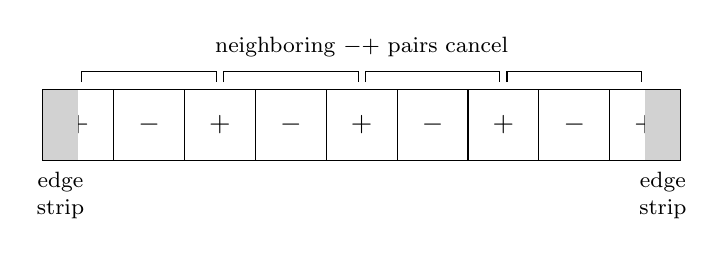
\begin{tikzpicture}[x=0.9cm, y=0.9cm]
  \foreach \i in {0,...,8} {
    \draw (\i,0) rectangle (\i+1,1);
    \ifodd\i \node at (\i+0.5,0.5) {$-$}; \else \node at (\i+0.5,0.5) {$+$}; \fi
  }
  \fill[gray!35] (0,0) rectangle (0.5,1);
  \fill[gray!35] (8.5,0) rectangle (9,1);
  \draw (0,0) rectangle (9,1);
  \foreach \i in {0.5,2.5,4.5,6.5} {
    \draw (\i+0.05,1.1) -- (\i+0.05,1.25) -- (\i+1.95,1.25) -- (\i+1.95,1.1);
  }
  \node[font=\footnotesize] at (4.5,1.6) {neighboring $-{}+$ pairs cancel};
  \node[font=\footnotesize, align=center] at (0.25,-0.5) {edge\\strip};
  \node[font=\footnotesize, align=center] at (8.75,-0.5) {edge\\strip};
\end{tikzpicture}
\caption{One row of half-wavelength regions of a subsonic mode. Pairs cancel; only
the unpaired strips at the edges (gray, and in 2D the corners) are left to radiate.}
\label{fig:edge_radiation}
\end{figure}

% ---------------------------------------------------------------------
\section{What the resonators change}

\subsection{They add small-$k$ states at $1270\,\mathrm{Hz}$}
At $1260\,\mathrm{Hz}$ the bare plate has no choice: every free motion has
$k = k_b = 31.8\,\mathrm{rad/m}$. The flat resonator branch
(Chapter~\ref{ch:local_resonance}) provides modes at about $1270\,\mathrm{Hz}$
for \emph{every} $\mathbf{k}$ in the Brillouin zone, including small $|\mathbf{k}|$
inside the radiation cone (Figure~\ref{fig:radiation_dispersion}). The resonators
do not smooth out the bare mode; they create a kind of mode that the bare plate
cannot have at this frequency.

\subsection{What a flat-branch mode looks like}
By Bloch's theorem (Chapter~\ref{ch:bloch}) a mode on the flat branch is
\begin{equation}
  w(\mathbf{x}) = e^{i\mathbf{k}\cdot\mathbf{x}}\; p(\mathbf{x}),
  \qquad p \text{ cell-periodic},
\end{equation}
a slowly varying envelope $e^{i\mathbf{k}\cdot\mathbf{x}}$ times the same cell
pattern $p$ in every cell.

\paragraph{The cell pattern near $\Gamma$.}
In the in-phase mode the resonator mass bounces on its spring and the plate cell
recoils. With the resonator amplitude $u$ and the mean plate displacement
$\bar w$ of the cell, momentum balance per cell (no external force) gives
\begin{equation}
  m\,u + \rho h A\, \bar w = 0
  \quad\Longrightarrow\quad
  \bar w = -\mu\, u = -0.25\,u .
\end{equation}
The whole cell moves opposite to the resonator with a quarter of its amplitude. On
top of that sits a local dimple under the attachment point, where the spring force
bends the plate (Figure~\ref{fig:cell_pattern}). The dimple is what lowers the
frequency from $f_r\sqrt{1+\mu} = 1342\,\mathrm{Hz}$ (rigid cell) to the FE value
of $1273\,\mathrm{Hz}$ (Chapter~\ref{ch:gap_position}).

\begin{figure}[htbp]
\centering
\begin{tikzpicture}[x=1cm, y=1cm, >={Stealth}]
  % undeformed plate (reference)
  \draw[gray, dashed] (0,0) -- (5,0);
  \node[gray, font=\footnotesize, left] at (0,0) {rest};
  % deformed plate: shifted down by 0.25 with a dimple at x = 2.5
  \draw[thick] plot[domain=0:5, samples=150] (\x, {-0.35 - 0.25*exp(-((\x-2.5)^2)/0.15)});
  % spring
  \draw (2.5,-0.6) -- (2.5,-0.45) -- (2.35,-0.35) -- (2.65,-0.15) -- (2.35,0.05)
        -- (2.65,0.25) -- (2.35,0.45) -- (2.5,0.55) -- (2.5,0.7);
  % mass
  \draw[fill=gray!30] (2.1,0.7) rectangle (2.9,1.2);
  \node[font=\footnotesize] at (2.5,0.95) {$m$};
  \draw[->, thick] (3.2,0.95) -- (3.2,1.55) node[right, font=\footnotesize] {$u$};
  \draw[->, thick] (4.4,-0.05) -- (4.4,-0.35) node[right, font=\footnotesize] {$\bar w = -\mu u$};
  \node[font=\footnotesize] at (1.0,-0.85) {one cell ($10\,\mathrm{cm}$)};
  \node[font=\footnotesize] at (3.6,-0.85) {dimple};
\end{tikzpicture}
\caption{Cell pattern of the in-phase mode near $\Gamma$ (exaggerated): the cell
moves down as a whole while the resonator moves up, with a local dimple at the
attachment point.}
\label{fig:cell_pattern}
\end{figure}

\paragraph{The finite plate.}
The 40 modes of the finite plate between $1246$ and $1282\,\mathrm{Hz}$ are
66--78\,\% resonator motion. Each repeats the cell pattern under a smooth envelope
that varies over the whole plate, like the low-order modes of a $10 \times 10$ grid
of masses. Split the plate motion into two parts (Figure~\ref{fig:smooth_ripple}):
\begin{itemize}
  \item the \textbf{smooth part}: cell means $\bar w$ times the envelope;
  \item the \textbf{ripple}: the dimples, repeated in every cell.
\end{itemize}

\begin{figure}[htbp]
\centering
\begin{tikzpicture}[x=1cm, y=1cm, >={Stealth}]
  % resonator amplitudes following the envelope sin(pi x / 10), 10 cells over 10 units
  \begin{scope}[yshift=3.6cm]
    \foreach \i in {0,...,9} {
      \pgfmathsetmacro{\amp}{0.7*sin((\i+0.5)*18)}
      \draw[->, thick] (\i+0.5,0) -- (\i+0.5,\amp);
    }
    \draw[gray] (0,0) -- (10,0);
    \node[font=\footnotesize, left] at (0,0.3) {resonators};
  \end{scope}
  % smooth part
  \begin{scope}[yshift=2.2cm]
    \draw[gray, dashed] (0,0) -- (10,0);
    \draw[thick] plot[domain=0:10, samples=100] (\x, {-0.5*sin(\x*18)});
    \node[font=\footnotesize, left, align=right] at (0,0) {smooth part\\ $k \approx \pi/L$};
  \end{scope}
  % ripple
  \begin{scope}[yshift=1.0cm]
    \draw[gray, dashed] (0,0) -- (10,0);
    \draw[thick] plot[domain=0:10, samples=400] (\x, {-0.2*sin(\x*18)*exp(-((\x-floor(\x)-0.5)^2)/0.02)});
    \node[font=\footnotesize, left, align=right] at (0,0) {ripple\\ $k \ge 2\pi/a$};
  \end{scope}
  % total
  \begin{scope}[yshift=-0.4cm]
    \draw[gray, dashed] (0,0) -- (10,0);
    \draw[thick] plot[domain=0:10, samples=400] (\x, {-0.5*sin(\x*18) - 0.2*sin(\x*18)*exp(-((\x-floor(\x)-0.5)^2)/0.02)});
    \node[font=\footnotesize, left] at (0,0) {plate};
  \end{scope}
  \draw[|<->|] (0,-1.3) -- (10,-1.3) node[midway, below, font=\footnotesize] {$L = 1\,\mathrm{m}$, 10 cells};
\end{tikzpicture}
\caption{A low-order cluster mode (side view, schematic). Top: resonator
amplitudes follow a smooth envelope. Below: the plate motion is a smooth part
(cell means, opposite to the resonators) plus a ripple of dimples, one per cell.}
\label{fig:smooth_ripple}
\end{figure}

\subsection{Which part radiates}
\begin{center}
\begin{tabular}{|l|p{0.28\textwidth}|p{0.18\textwidth}|p{0.27\textwidth}|}
\hline
Part & Wavenumbers & vs.\ $k_\mathrm{air} = 23.1\,\mathrm{rad/m}$ & Radiates? \\
\hline
smooth part & envelope: $m\pi/L = 3.1, 6.3, 9.4, \dots\,\mathrm{rad/m}$ & inside the cone for low orders & yes: $+$ and $-$ regions tens of cm apart \\
ripple & $\ge 2\pi/a = 62.8\,\mathrm{rad/m}$ & far outside & no: decay length $1/\sqrt{62.8^2 - 23.1^2}\,\mathrm{m} = 1.7\,\mathrm{cm}$ \\
\hline
\end{tabular}
\end{center}
In the extreme case of a uniform envelope ($\mathbf{k} = 0$), all cell means move in
phase and the plate acts as a piston. A rough estimate (not computed): envelope
orders up to $m \approx 7$ satisfy $m\pi/L < 23.1\,\mathrm{rad/m}$ on the
$1\,\mathrm{m}$ plate, which fits the observation that most, but not all, cluster
modes radiate strongly.

\paragraph{Why the plate simply follows the resonators.}
For a force pattern with wavenumber $k$ the plate responds (Kirchhoff, undamped) with
\begin{equation}
  \hat w(k) = \frac{\hat F(k)}{D k^4 - \rho h\,\omega^2}
  \;\overset{k \ll k_b}{\approx}\; -\frac{\hat F(k)}{\rho h\,\omega^2} .
\end{equation}
At small $k$ the bending stiffness $D k^4$ is negligible; the plate acts like a mass
and moves with whatever smooth pattern the resonators impose. The plate goes where
the resonators push it, and they push smoothly.

\subsection{The numbers}
From the modal analysis of the finite plate (open check (b),
\texttt{check\_finite\_plate\_modes.py}):
\begin{center}
\begin{tabular}{|l|l|}
\hline
Modes & Radiation efficiency $\sigma$ \\
\hline
bare plate, near $1260\,\mathrm{Hz}$ & $0.003$--$0.014$ \\
cluster $1246$--$1282\,\mathrm{Hz}$, $2\times 2$ shear rule & $0.35$--$0.90$ \\
cluster, full $3\times 3$ shear rule & $0.54$--$0.80$ \\
\hline
\end{tabular}
\end{center}
Per unit velocity the cluster modes radiate about $20\,\mathrm{dB}$ more than the bare
modes. In Eq.~\eqref{eq:il_split} the efficiency term is then about
$10\log_{10}(0.01/0.5) \approx -17\,\mathrm{dB}$, which the velocity term cannot
compensate: the IL dips to about $-14\,\mathrm{dB}$. (Rough: in the forced response
several modes overlap, so the modal $\sigma$ values only bracket the effective one.)
With the full $3\times 3$ shear rule, now used throughout, the dip is
$-13.9\,\mathrm{dB}$ at $1267\,\mathrm{Hz}$.

\paragraph{Inside a gap: the $600\,\mathrm{Hz}$ tuning.} The same mechanism can reach into
a gap. With $f_r = 600\,\mathrm{Hz}$ ($\tau = 0.5$, Bloch gap $578$--$662\,\mathrm{Hz}$) the
IL turns negative from $633\,\mathrm{Hz}$ on, about $65\,\%$ into the gap. Averaged over
$628$--$662\,\mathrm{Hz}$: IL $-7.4\,\mathrm{dB}$ = velocity term $+7.8\,\mathrm{dB}$ +
efficiency term $-15.2\,\mathrm{dB}$. The plate does move less, as the gap requires, but the
remaining motion radiates far better. At this tuning the upper gap edge \emph{is} the
resonator band at $\Gamma$ (small $k$, supersonic), and the bare plate, four times below
$f_c$, radiates very poorly. At $1200\,\mathrm{Hz}$ the upper edge is the sin pattern at
$X$, which is subsonic ($31.4$ against $21.9\,\mathrm{rad/m}$), and the efficiency term
inside the gap stays near $-3\,\mathrm{dB}$.

% ---------------------------------------------------------------------
\section{Summary}
\begin{enumerate}
  \item Below $f_c \approx 2.4\,\mathrm{kHz}$ free bending waves are subsonic
        ($k_b > k_\mathrm{air}$); the air short-circuits between neighboring crests
        and troughs, and only edges and corners radiate ($\sigma \sim 0.01$).
  \item The flat resonator branch provides modes at about $1270\,\mathrm{Hz}$ for all
        $\mathbf{k}$, including small $\mathbf{k}$ inside the radiation cone.
  \item In these modes the plate moves as cell means (opposite to the resonators,
        $\bar w = -\mu u$) under a smooth envelope, plus a ripple of dimples. The
        smooth part is supersonic and radiates ($\sigma \sim 0.5$); the ripple does not.
  \item The plate does not move more, it moves in a shape the air cannot short-circuit:
        the efficiency term of the IL is about $-17\,\mathrm{dB}$, giving the
        $-14\,\mathrm{dB}$ dip.
\end{enumerate}

% ---------------------------------------------------------------------
\section{Check questions with answers}

\paragraph{Question 1.} \emph{Would the bare plate radiate better at
$2000\,\mathrm{Hz}$ than at $1260\,\mathrm{Hz}$? Use the wavenumbers.}

\emph{Answer.} Yes. $k_b \propto \sqrt{f}$: $k_b(2000) = 31.8\sqrt{2000/1260} =
40.1\,\mathrm{rad/m}$, while $k_\mathrm{air}(2000) = 2\pi\cdot 2000/343 =
36.6\,\mathrm{rad/m}$. Still subsonic, but much closer to coincidence: the decay
length grows from $4.6\,\mathrm{cm}$ to $1/\sqrt{40.1^2 - 36.6^2}\,\mathrm{m} \approx
6.1\,\mathrm{cm}$, and crest and trough are $7.8\,\mathrm{cm}$ apart against
$8.6\,\mathrm{cm}$ covered by sound in half a period. The short circuit becomes
incomplete; $\sigma$ rises towards its maximum near $f_c$.

\paragraph{Question 2.} \emph{The resonators push hardest right at the attachment
points, where the dimples are. Why does that motion not radiate?}

\emph{Answer.} The dimples repeat with the lattice period, so their wavenumbers are at
least $2\pi/a = 62.8\,\mathrm{rad/m}$, almost three times $k_\mathrm{air}$. Their
pressure decays with a length of $1.7\,\mathrm{cm}$: each dimple is short-circuited by
the surrounding plate, which moves the other way. Only the cell means, collected under
a smooth envelope, reach the far field.

\paragraph{Question 3.} \emph{Resonators tuned to $3\,\mathrm{kHz}$, above $f_c$: would
the same IL dip appear at their flat branch?}

\emph{Answer (expectation, not computed).} Much weaker. Above $f_c$ the bare plate's
free waves are already supersonic and radiate with $\sigma \approx 1$. The flat branch
cannot raise $\sigma$ much further, so the efficiency term of
Eq.~\eqref{eq:il_split} is small, and the IL is governed by the velocity term. The dip
is a below-coincidence effect.

% =====================================================================

\chapter{Sound radiation: why the resonator lattice can make the plate louder}
\label{ch:radiation}

The finite $1 \times 1\,\mathrm{m}$ plate with $10 \times 10$ resonators on the
$0.1\,\mathrm{m}$ lattice ($f_r = 1.2\,\mathrm{kHz}$, $\mu = 0.25$) shows two
features in the insertion loss (IL) of the radiated power:
\begin{itemize}
  \item a peak of about $+13\,\mathrm{dB}$ inside the Bloch gap
        $1031$--$1195\,\mathrm{Hz}$ (Chapter~\ref{ch:complex_k}: evanescent
        waves);
  \item a dip of about $-14\,\mathrm{dB}$ at about $1260\,\mathrm{Hz}$, right at
        the flat resonator branch: \emph{with} resonators the plate radiates more
        than without.
\end{itemize}
This chapter explains the dip. The short version: the resonators do not make the
plate move more, they make it move in a shape that the air cannot short-circuit.

\begin{center}
\begin{tabular}{|l|p{0.5\textwidth}|l|}
\hline
Symbol & Meaning & Value at $1260\,\mathrm{Hz}$ \\
\hline
$c$, $\rho_0$ & speed of sound, density of air & $343\,\mathrm{m/s}$, $1.2\,\mathrm{kg/m^3}$ \\
$k_\mathrm{air} = \omega/c$ & acoustic wavenumber & $23.1\,\mathrm{rad/m}$ \\
$\lambda_\mathrm{air} = 2\pi/k_\mathrm{air}$ & acoustic wavelength & $27.2\,\mathrm{cm}$ \\
$D = E h^3/(12(1-\nu^2))$ & bending stiffness & $2404\,\mathrm{N\,m}$ \\
$k_b = (\omega^2 \rho h/D)^{1/4}$ & free bending wavenumber (Kirchhoff) & $31.8\,\mathrm{rad/m}$ \\
$\lambda_b = 2\pi/k_b$ & bending wavelength & $19.8\,\mathrm{cm}$ \\
$c_b = \omega/k_b$ & phase (trace) speed of the bending wave & $249\,\mathrm{m/s}$ \\
$k_x$ & wavenumber of a plate pattern along the surface & -- \\
$k_z$ & wavenumber of the air field normal to the plate & -- \\
$S$ & plate area & $1\,\mathrm{m^2}$ \\
$\langle v^2 \rangle$ & mean square normal velocity, averaged over the plate & -- \\
$W$ & radiated sound power & -- \\
$\sigma$ & radiation efficiency & -- \\
$f_c$ & critical (coincidence) frequency & $\approx 2.4\,\mathrm{kHz}$ \\
\hline
\end{tabular}
\end{center}

% ---------------------------------------------------------------------
\section{Radiation efficiency}

The radiated power is written as
\begin{equation}
  W = \rho_0 c\, S\, \langle v^2 \rangle\, \sigma .
  \label{eq:radiation_efficiency}
\end{equation}
$\rho_0 c S \langle v^2 \rangle$ is the power a rigid piston of the same area and
the same mean square velocity would radiate at high frequency. $\sigma$ says how
much of that the actual vibration pattern achieves: $\sigma \approx 1$ for a
piston-like pattern, $\sigma \ll 1$ for a pattern that ``wastes'' its motion.

Since the IL compares the radiated power of the bare plate with that of the plate
with resonators, Eq.~\eqref{eq:radiation_efficiency} splits it into two parts:
\begin{equation}
  \mathrm{IL} = 10\log_{10}\frac{W_\mathrm{bare}}{W_\mathrm{res}}
  = \underbrace{10\log_{10}\frac{\langle v^2\rangle_\mathrm{bare}}{\langle v^2\rangle_\mathrm{res}}}_{\text{velocity term}}
  + \underbrace{10\log_{10}\frac{\sigma_\mathrm{bare}}{\sigma_\mathrm{res}}}_{\text{efficiency term}} .
  \label{eq:il_split}
\end{equation}
The resonators can make the velocity term positive (less motion) and still produce
a negative IL if they raise $\sigma$ enough. This is what happens at the flat branch.

% ---------------------------------------------------------------------
\section{Subsonic and supersonic patterns}

\subsection{Trace matching}
Let the plate vibrate with a pattern $v(x) = \hat v\, e^{i k_x x}$ along its surface
(time factor $e^{i\omega t}$). At the surface the air must move with the plate, so
the air field has the same $k_x$. In air every field obeys the wave equation,
which for a plane-wave component $e^{i(k_x x + k_z z)}$ means
\begin{equation}
  k_x^2 + k_z^2 = k_\mathrm{air}^2
  \quad\Longrightarrow\quad
  k_z = \sqrt{k_\mathrm{air}^2 - k_x^2} .
\end{equation}
Two cases:
\begin{itemize}
  \item $k_x < k_\mathrm{air}$: $k_z$ is real, a plane wave leaves the plate at the
        angle $\alpha$ from the normal with $\sin\alpha = k_x/k_\mathrm{air}$. Power
        is carried away.
  \item $k_x > k_\mathrm{air}$: $k_z = \pm i\sqrt{k_x^2 - k_\mathrm{air}^2}$ is
        imaginary, the pressure decays like
        $e^{-z\sqrt{k_x^2 - k_\mathrm{air}^2}}$ away from the plate. This is a
        \emph{near field}; it carries no power.
\end{itemize}

\subsection{Why ``supersonic'' means \emph{small} $k$}
The names refer to the \emph{phase speed} of the pattern along the plate,
$c_\mathrm{trace} = \omega/k_x$, not to the material velocity (which is always tiny).
At fixed $\omega$ a larger wavenumber means a shorter wavelength and a slower
pattern:
\begin{equation}
  k_x < k_\mathrm{air} \;\Longleftrightarrow\; \frac{\omega}{k_x} > c
  \quad\text{(supersonic)},
  \qquad
  k_x > k_\mathrm{air} \;\Longleftrightarrow\; \frac{\omega}{k_x} < c
  \quad\text{(subsonic)} .
\end{equation}
For the bare plate at $1260\,\mathrm{Hz}$, $k_b = 31.8 > 23.1 = k_\mathrm{air}$:
the free bending wave is subsonic ($c_b = 249\,\mathrm{m/s} < 343\,\mathrm{m/s}$).
Its pressure decays with the length
$1/\sqrt{31.8^2 - 23.1^2}\,\mathrm{m} = 1/21.9\,\mathrm{m} \approx 4.6\,\mathrm{cm}$.

\subsection{The critical frequency}
Bending waves are dispersive: $f = \frac{1}{2\pi}\sqrt{D/(\rho h)}\, k_b^2$, so
$k_b \propto \sqrt{f}$, while $k_\mathrm{air} \propto f$. The air line overtakes the
bending curve at the critical frequency
\begin{equation}
  f_c = \frac{c^2}{2\pi}\sqrt{\frac{\rho h}{D}} \approx 2.4\,\mathrm{kHz}
  \quad (5\,\mathrm{mm} \text{ steel; RM gives about } 2.45\,\mathrm{kHz}).
\end{equation}
Below $f_c$ free bending waves are subsonic, above it supersonic.
Figure~\ref{fig:radiation_dispersion} shows both curves.

\begin{figure}[htbp]
\centering
\begin{tikzpicture}[x=0.11cm, y=0.0019cm, >={Stealth}]
  % radiation cone: k < k_air(f), i.e. left of the air line
  \fill[gray!18] (0,0) -- (54.9,3000) -- (0,3000) -- cycle;
  \node[align=left, font=\footnotesize] at (11,2550) {radiation cone\\ $k < k_\mathrm{air}$\\ (supersonic)};
  % axes
  \draw[->] (0,0) -- (57,0) node[below left] {$k$ (rad/m)};
  \draw[->] (0,0) -- (0,3250) node[above] {$f$ (Hz)};
  \foreach \kk in {10,20,30,40,50} \draw (\kk,0) -- (\kk,-60) node[below, font=\scriptsize] {\kk};
  \foreach \ff in {1000,2000,3000} \draw (0,\ff) -- (-1,\ff) node[left, font=\scriptsize] {\ff};
  % air line f = c k / (2 pi) = 54.6 k
  \draw[thick, dashed] (0,0) -- (54.9,3000) node[above, font=\footnotesize] {air: $f = c k/2\pi$};
  % bare bending curve f = 1.245 k^2
  \draw[thick] plot[domain=0:49, samples=60] (\x, {1.245*\x*\x});
  \node[font=\footnotesize, right] at (47,2500) {bare plate};
  % flat resonator branch (schematic)
  \draw[very thick, gray] (0,1270) -- (44.4,1270);
  \node[font=\footnotesize, gray, right] at (44.4,1270) {flat resonator branch};
  % 1260 Hz markers
  \draw[dotted] (0,1260) -- (31.8,1260);
  \draw[dotted] (23.1,0) -- (23.1,1260);
  \draw[dotted] (31.8,0) -- (31.8,1260);
  \fill (23.1,1260) circle (1.2pt);
  \fill (31.8,1260) circle (1.2pt);
  \node[font=\scriptsize, below] at (21.5,500) {$k_\mathrm{air}$};
  \node[font=\scriptsize, below] at (34,500) {$k_b$};
  % critical frequency
  \fill (43.9,2396) circle (1.5pt) node[right, font=\footnotesize] {$f_c$};
\end{tikzpicture}
\caption{Bending curve (Kirchhoff, $5\,\mathrm{mm}$ steel) and air line. Shaded:
patterns with $k < k_\mathrm{air}$, which radiate. At $1260\,\mathrm{Hz}$ the bare
plate only has $k_b = 31.8\,\mathrm{rad/m}$, outside the cone. The flat resonator
branch (schematic, gray) offers states at about $1270\,\mathrm{Hz}$ for every
$\mathbf{k}$, including small $k$ inside the cone.}
\label{fig:radiation_dispersion}
\end{figure}

% ---------------------------------------------------------------------
\section{The acoustic short circuit}

\subsection{The time argument}
A crest of the plate pushes air out, the neighboring trough sucks air in. The
pushed air can flow sideways into the trough if it gets there before the plate
reverses, i.e.\ within half a period $T/2$. Disturbances in air travel at $c$, so
in that time they cover
\begin{equation}
  c\,\frac{T}{2} = \frac{\lambda_\mathrm{air}}{2} .
\end{equation}
The trough is $\lambda_b/2$ away. The short circuit works if
\begin{equation}
  \frac{\lambda_b}{2} < \frac{\lambda_\mathrm{air}}{2}
  \;\Longleftrightarrow\; \lambda_b < \lambda_\mathrm{air}
  \;\Longleftrightarrow\; k_b > k_\mathrm{air}
  \;\Longleftrightarrow\; \text{subsonic} .
\end{equation}
The time argument is the trace-matching condition in words. At $1260\,\mathrm{Hz}$
the trough is $9.9\,\mathrm{cm}$ away and sound covers $13.6\,\mathrm{cm}$ in half a
period: the air gets there in time (Figure~\ref{fig:short_circuit}).

\begin{figure}[htbp]
\centering
\begin{tikzpicture}[x=1cm, y=1cm, >={Stealth}]
  % plate: half wavelength = 1 unit = 9.9 cm
  \draw[thick] plot[domain=0:8, samples=200] (\x, {0.3*sin(\x*180)});
  \foreach \xx in {0.5,2.5,4.5,6.5} \node[font=\footnotesize] at (\xx,-0.2) {$+$};
  \foreach \xx in {1.5,3.5,5.5,7.5} \node[font=\footnotesize] at (\xx,0.2) {$-$};
  % sideways air flow from crests into troughs
  \foreach \xx in {0.5,2.5,4.5,6.5} {
    \draw[->, gray] (\xx+0.1,0.55) -- (\xx+0.9,0.55);
    \draw[->, gray] (\xx-0.1,0.55) -- (\xx-0.9,0.55);
  }
  % distances
  \draw[|<->|] (0.5,-0.75) -- (1.5,-0.75) node[midway, below, font=\footnotesize] {$\lambda_b/2 = 9.9\,\mathrm{cm}$};
  \draw[|<->|] (4.5,-0.75) -- (5.87,-0.75) node[midway, below, font=\footnotesize] {$\lambda_\mathrm{air}/2 = 13.6\,\mathrm{cm}$};
  \node[font=\footnotesize, gray] at (4,1.0) {air sloshes sideways: short circuit, almost nothing leaves};
\end{tikzpicture}
\caption{Bare plate at $1260\,\mathrm{Hz}$ (side view). In half a period, sound
travels farther ($13.6\,\mathrm{cm}$) than the distance from crest to trough
($9.9\,\mathrm{cm}$): the air flows sideways instead of outward.}
\label{fig:short_circuit}
\end{figure}

\subsection{The same in the near field}
Figure~\ref{fig:near_far} shows what the trace-matching result means for the
pressure. On the left, the subsonic ripple: the pressure pattern above the plate
dies out within a few centimeters. On the right, a supersonic pattern: wavefronts
leave the plate at the angle $\alpha$.

\begin{figure}[htbp]
\centering
\begin{tikzpicture}[x=1cm, y=1cm, >={Stealth}]
  % left: subsonic, 1 unit = 9.9 cm, decay length 0.46 units
  \begin{scope}
    \draw[thick] plot[domain=0:4, samples=120] (\x, {0.3*sin(\x*180)});
    \foreach \zz in {0.4,0.8,1.2,1.6} {
      \draw[gray] plot[domain=0:4, samples=120] (\x, {\zz + 0.3*exp(-\zz/0.46)*sin(\x*180)});
    }
    \node[font=\footnotesize, align=center] at (2,2.3) {subsonic ($k_x = 31.8\,\mathrm{rad/m}$)\\ pressure dies out within $\sim 5\,\mathrm{cm}$};
  \end{scope}
  % right: supersonic, long wavelength, slanted wavefronts
  \begin{scope}[xshift=5.5cm]
    \draw[thick] plot[domain=0:4, samples=120] (\x, {0.3*sin(\x*45)});
    \foreach \s in {0,0.6,1.2,1.8,2.4} {
      \draw[gray] (\s,0.35) -- (\s+1.2,1.85);
    }
    \draw[->] (2.2,0.6) -- (2.95,1.2) node[right, font=\footnotesize] {sound};
    \node[font=\footnotesize, align=center] at (2,2.3) {supersonic ($k_x < k_\mathrm{air}$)\\ wavefronts leave at $\sin\alpha = k_x/k_\mathrm{air}$};
  \end{scope}
\end{tikzpicture}
\caption{Left: lines of equal height show the pressure amplitude above a subsonic
ripple, decaying like $e^{-z/4.6\,\mathrm{cm}}$. Right: a long-wavelength
(supersonic) pattern sends plane waves into the air.}
\label{fig:near_far}
\end{figure}

\subsection{Why the bare finite plate radiates at all}
On a finite plate, every $+$ region of a subsonic mode has a $-$ neighbor that
cancels it, except where the pattern ends. The uncanceled strips along the edges
and the uncanceled corner cells radiate (Figure~\ref{fig:edge_radiation}). Their
area is small compared with the plate, so $\sigma \ll 1$. For the bare modes near
$1260\,\mathrm{Hz}$ the modal analysis (open check (b)) gave
$\sigma = 0.003$--$0.014$.

\begin{figure}[htbp]
\centering
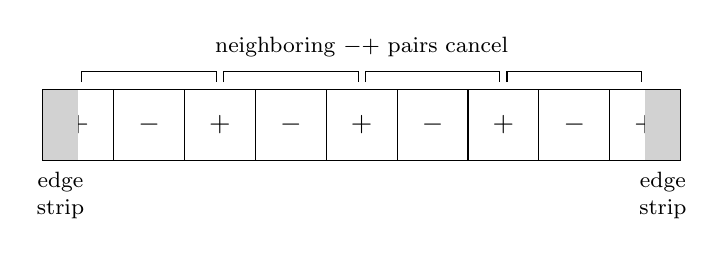
\begin{tikzpicture}[x=0.9cm, y=0.9cm]
  \foreach \i in {0,...,8} {
    \draw (\i,0) rectangle (\i+1,1);
    \ifodd\i \node at (\i+0.5,0.5) {$-$}; \else \node at (\i+0.5,0.5) {$+$}; \fi
  }
  \fill[gray!35] (0,0) rectangle (0.5,1);
  \fill[gray!35] (8.5,0) rectangle (9,1);
  \draw (0,0) rectangle (9,1);
  \foreach \i in {0.5,2.5,4.5,6.5} {
    \draw (\i+0.05,1.1) -- (\i+0.05,1.25) -- (\i+1.95,1.25) -- (\i+1.95,1.1);
  }
  \node[font=\footnotesize] at (4.5,1.6) {neighboring $-{}+$ pairs cancel};
  \node[font=\footnotesize, align=center] at (0.25,-0.5) {edge\\strip};
  \node[font=\footnotesize, align=center] at (8.75,-0.5) {edge\\strip};
\end{tikzpicture}
\caption{One row of half-wavelength regions of a subsonic mode. Pairs cancel; only
the unpaired strips at the edges (gray, and in 2D the corners) are left to radiate.}
\label{fig:edge_radiation}
\end{figure}

% ---------------------------------------------------------------------
\section{What the resonators change}

\subsection{They add small-$k$ states at $1270\,\mathrm{Hz}$}
At $1260\,\mathrm{Hz}$ the bare plate has no choice: every free motion has
$k = k_b = 31.8\,\mathrm{rad/m}$. The flat resonator branch
(Chapter~\ref{ch:local_resonance}) provides modes at about $1270\,\mathrm{Hz}$
for \emph{every} $\mathbf{k}$ in the Brillouin zone, including small $|\mathbf{k}|$
inside the radiation cone (Figure~\ref{fig:radiation_dispersion}). The resonators
do not smooth out the bare mode; they create a kind of mode that the bare plate
cannot have at this frequency.

\subsection{What a flat-branch mode looks like}
By Bloch's theorem (Chapter~\ref{ch:bloch}) a mode on the flat branch is
\begin{equation}
  w(\mathbf{x}) = e^{i\mathbf{k}\cdot\mathbf{x}}\; p(\mathbf{x}),
  \qquad p \text{ cell-periodic},
\end{equation}
a slowly varying envelope $e^{i\mathbf{k}\cdot\mathbf{x}}$ times the same cell
pattern $p$ in every cell.

\paragraph{The cell pattern near $\Gamma$.}
In the in-phase mode the resonator mass bounces on its spring and the plate cell
recoils. With the resonator amplitude $u$ and the mean plate displacement
$\bar w$ of the cell, momentum balance per cell (no external force) gives
\begin{equation}
  m\,u + \rho h A\, \bar w = 0
  \quad\Longrightarrow\quad
  \bar w = -\mu\, u = -0.25\,u .
\end{equation}
The whole cell moves opposite to the resonator with a quarter of its amplitude. On
top of that sits a local dimple under the attachment point, where the spring force
bends the plate (Figure~\ref{fig:cell_pattern}). The dimple is what lowers the
frequency from $f_r\sqrt{1+\mu} = 1342\,\mathrm{Hz}$ (rigid cell) to the FE value
of $1273\,\mathrm{Hz}$ (Chapter~\ref{ch:gap_position}).

\begin{figure}[htbp]
\centering
\begin{tikzpicture}[x=1cm, y=1cm, >={Stealth}]
  % undeformed plate (reference)
  \draw[gray, dashed] (0,0) -- (5,0);
  \node[gray, font=\footnotesize, left] at (0,0) {rest};
  % deformed plate: shifted down by 0.25 with a dimple at x = 2.5
  \draw[thick] plot[domain=0:5, samples=150] (\x, {-0.35 - 0.25*exp(-((\x-2.5)^2)/0.15)});
  % spring
  \draw (2.5,-0.6) -- (2.5,-0.45) -- (2.35,-0.35) -- (2.65,-0.15) -- (2.35,0.05)
        -- (2.65,0.25) -- (2.35,0.45) -- (2.5,0.55) -- (2.5,0.7);
  % mass
  \draw[fill=gray!30] (2.1,0.7) rectangle (2.9,1.2);
  \node[font=\footnotesize] at (2.5,0.95) {$m$};
  \draw[->, thick] (3.2,0.95) -- (3.2,1.55) node[right, font=\footnotesize] {$u$};
  \draw[->, thick] (4.4,-0.05) -- (4.4,-0.35) node[right, font=\footnotesize] {$\bar w = -\mu u$};
  \node[font=\footnotesize] at (1.0,-0.85) {one cell ($10\,\mathrm{cm}$)};
  \node[font=\footnotesize] at (3.6,-0.85) {dimple};
\end{tikzpicture}
\caption{Cell pattern of the in-phase mode near $\Gamma$ (exaggerated): the cell
moves down as a whole while the resonator moves up, with a local dimple at the
attachment point.}
\label{fig:cell_pattern}
\end{figure}

\paragraph{The finite plate.}
The 40 modes of the finite plate between $1246$ and $1282\,\mathrm{Hz}$ are
66--78\,\% resonator motion. Each repeats the cell pattern under a smooth envelope
that varies over the whole plate, like the low-order modes of a $10 \times 10$ grid
of masses. Split the plate motion into two parts (Figure~\ref{fig:smooth_ripple}):
\begin{itemize}
  \item the \textbf{smooth part}: cell means $\bar w$ times the envelope;
  \item the \textbf{ripple}: the dimples, repeated in every cell.
\end{itemize}

\begin{figure}[htbp]
\centering
\begin{tikzpicture}[x=1cm, y=1cm, >={Stealth}]
  % resonator amplitudes following the envelope sin(pi x / 10), 10 cells over 10 units
  \begin{scope}[yshift=3.6cm]
    \foreach \i in {0,...,9} {
      \pgfmathsetmacro{\amp}{0.7*sin((\i+0.5)*18)}
      \draw[->, thick] (\i+0.5,0) -- (\i+0.5,\amp);
    }
    \draw[gray] (0,0) -- (10,0);
    \node[font=\footnotesize, left] at (0,0.3) {resonators};
  \end{scope}
  % smooth part
  \begin{scope}[yshift=2.2cm]
    \draw[gray, dashed] (0,0) -- (10,0);
    \draw[thick] plot[domain=0:10, samples=100] (\x, {-0.5*sin(\x*18)});
    \node[font=\footnotesize, left, align=right] at (0,0) {smooth part\\ $k \approx \pi/L$};
  \end{scope}
  % ripple
  \begin{scope}[yshift=1.0cm]
    \draw[gray, dashed] (0,0) -- (10,0);
    \draw[thick] plot[domain=0:10, samples=400] (\x, {-0.2*sin(\x*18)*exp(-((\x-floor(\x)-0.5)^2)/0.02)});
    \node[font=\footnotesize, left, align=right] at (0,0) {ripple\\ $k \ge 2\pi/a$};
  \end{scope}
  % total
  \begin{scope}[yshift=-0.4cm]
    \draw[gray, dashed] (0,0) -- (10,0);
    \draw[thick] plot[domain=0:10, samples=400] (\x, {-0.5*sin(\x*18) - 0.2*sin(\x*18)*exp(-((\x-floor(\x)-0.5)^2)/0.02)});
    \node[font=\footnotesize, left] at (0,0) {plate};
  \end{scope}
  \draw[|<->|] (0,-1.3) -- (10,-1.3) node[midway, below, font=\footnotesize] {$L = 1\,\mathrm{m}$, 10 cells};
\end{tikzpicture}
\caption{A low-order cluster mode (side view, schematic). Top: resonator
amplitudes follow a smooth envelope. Below: the plate motion is a smooth part
(cell means, opposite to the resonators) plus a ripple of dimples, one per cell.}
\label{fig:smooth_ripple}
\end{figure}

\subsection{Which part radiates}
\begin{center}
\begin{tabular}{|l|p{0.28\textwidth}|p{0.18\textwidth}|p{0.27\textwidth}|}
\hline
Part & Wavenumbers & vs.\ $k_\mathrm{air} = 23.1\,\mathrm{rad/m}$ & Radiates? \\
\hline
smooth part & envelope: $m\pi/L = 3.1, 6.3, 9.4, \dots\,\mathrm{rad/m}$ & inside the cone for low orders & yes: $+$ and $-$ regions tens of cm apart \\
ripple & $\ge 2\pi/a = 62.8\,\mathrm{rad/m}$ & far outside & no: decay length $1/\sqrt{62.8^2 - 23.1^2}\,\mathrm{m} = 1.7\,\mathrm{cm}$ \\
\hline
\end{tabular}
\end{center}
In the extreme case of a uniform envelope ($\mathbf{k} = 0$), all cell means move in
phase and the plate acts as a piston. A rough estimate (not computed): envelope
orders up to $m \approx 7$ satisfy $m\pi/L < 23.1\,\mathrm{rad/m}$ on the
$1\,\mathrm{m}$ plate, which fits the observation that most, but not all, cluster
modes radiate strongly.

\paragraph{Why the plate simply follows the resonators.}
For a force pattern with wavenumber $k$ the plate responds (Kirchhoff, undamped) with
\begin{equation}
  \hat w(k) = \frac{\hat F(k)}{D k^4 - \rho h\,\omega^2}
  \;\overset{k \ll k_b}{\approx}\; -\frac{\hat F(k)}{\rho h\,\omega^2} .
\end{equation}
At small $k$ the bending stiffness $D k^4$ is negligible; the plate acts like a mass
and moves with whatever smooth pattern the resonators impose. The plate goes where
the resonators push it, and they push smoothly.

\subsection{The numbers}
From the modal analysis of the finite plate (open check (b),
\texttt{check\_finite\_plate\_modes.py}):
\begin{center}
\begin{tabular}{|l|l|}
\hline
Modes & Radiation efficiency $\sigma$ \\
\hline
bare plate, near $1260\,\mathrm{Hz}$ & $0.003$--$0.014$ \\
cluster $1246$--$1282\,\mathrm{Hz}$, $2\times 2$ shear rule & $0.35$--$0.90$ \\
cluster, full $3\times 3$ shear rule & $0.54$--$0.80$ \\
\hline
\end{tabular}
\end{center}
Per unit velocity the cluster modes radiate about $20\,\mathrm{dB}$ more than the bare
modes. In Eq.~\eqref{eq:il_split} the efficiency term is then about
$10\log_{10}(0.01/0.5) \approx -17\,\mathrm{dB}$, which the velocity term cannot
compensate: the IL dips to about $-14\,\mathrm{dB}$. (Rough: in the forced response
several modes overlap, so the modal $\sigma$ values only bracket the effective one.)
With the full $3\times 3$ shear rule, now used throughout, the dip is
$-13.9\,\mathrm{dB}$ at $1267\,\mathrm{Hz}$.

\paragraph{Inside a gap: the $600\,\mathrm{Hz}$ tuning.} The same mechanism can reach into
a gap. With $f_r = 600\,\mathrm{Hz}$ ($\tau = 0.5$, Bloch gap $578$--$662\,\mathrm{Hz}$) the
IL turns negative from $633\,\mathrm{Hz}$ on, about $65\,\%$ into the gap. Averaged over
$628$--$662\,\mathrm{Hz}$: IL $-7.4\,\mathrm{dB}$ = velocity term $+7.8\,\mathrm{dB}$ +
efficiency term $-15.2\,\mathrm{dB}$. The plate does move less, as the gap requires, but the
remaining motion radiates far better. At this tuning the upper gap edge \emph{is} the
resonator band at $\Gamma$ (small $k$, supersonic), and the bare plate, four times below
$f_c$, radiates very poorly. At $1200\,\mathrm{Hz}$ the upper edge is the sin pattern at
$X$, which is subsonic ($31.4$ against $21.9\,\mathrm{rad/m}$), and the efficiency term
inside the gap stays near $-3\,\mathrm{dB}$.

% ---------------------------------------------------------------------
\section{Summary}
\begin{enumerate}
  \item Below $f_c \approx 2.4\,\mathrm{kHz}$ free bending waves are subsonic
        ($k_b > k_\mathrm{air}$); the air short-circuits between neighboring crests
        and troughs, and only edges and corners radiate ($\sigma \sim 0.01$).
  \item The flat resonator branch provides modes at about $1270\,\mathrm{Hz}$ for all
        $\mathbf{k}$, including small $\mathbf{k}$ inside the radiation cone.
  \item In these modes the plate moves as cell means (opposite to the resonators,
        $\bar w = -\mu u$) under a smooth envelope, plus a ripple of dimples. The
        smooth part is supersonic and radiates ($\sigma \sim 0.5$); the ripple does not.
  \item The plate does not move more, it moves in a shape the air cannot short-circuit:
        the efficiency term of the IL is about $-17\,\mathrm{dB}$, giving the
        $-14\,\mathrm{dB}$ dip.
\end{enumerate}

% ---------------------------------------------------------------------
\section{Check questions with answers}

\paragraph{Question 1.} \emph{Would the bare plate radiate better at
$2000\,\mathrm{Hz}$ than at $1260\,\mathrm{Hz}$? Use the wavenumbers.}

\emph{Answer.} Yes. $k_b \propto \sqrt{f}$: $k_b(2000) = 31.8\sqrt{2000/1260} =
40.1\,\mathrm{rad/m}$, while $k_\mathrm{air}(2000) = 2\pi\cdot 2000/343 =
36.6\,\mathrm{rad/m}$. Still subsonic, but much closer to coincidence: the decay
length grows from $4.6\,\mathrm{cm}$ to $1/\sqrt{40.1^2 - 36.6^2}\,\mathrm{m} \approx
6.1\,\mathrm{cm}$, and crest and trough are $7.8\,\mathrm{cm}$ apart against
$8.6\,\mathrm{cm}$ covered by sound in half a period. The short circuit becomes
incomplete; $\sigma$ rises towards its maximum near $f_c$.

\paragraph{Question 2.} \emph{The resonators push hardest right at the attachment
points, where the dimples are. Why does that motion not radiate?}

\emph{Answer.} The dimples repeat with the lattice period, so their wavenumbers are at
least $2\pi/a = 62.8\,\mathrm{rad/m}$, almost three times $k_\mathrm{air}$. Their
pressure decays with a length of $1.7\,\mathrm{cm}$: each dimple is short-circuited by
the surrounding plate, which moves the other way. Only the cell means, collected under
a smooth envelope, reach the far field.

\paragraph{Question 3.} \emph{Resonators tuned to $3\,\mathrm{kHz}$, above $f_c$: would
the same IL dip appear at their flat branch?}

\emph{Answer (expectation, not computed).} Much weaker. Above $f_c$ the bare plate's
free waves are already supersonic and radiate with $\sigma \approx 1$. The flat branch
cannot raise $\sigma$ much further, so the efficiency term of
Eq.~\eqref{eq:il_split} is small, and the IL is governed by the velocity term. The dip
is a below-coincidence effect.

% =====================================================================

\chapter{Sound radiation: why the resonator lattice can make the plate louder}
\label{ch:radiation}

The finite $1 \times 1\,\mathrm{m}$ plate with $10 \times 10$ resonators on the
$0.1\,\mathrm{m}$ lattice ($f_r = 1.2\,\mathrm{kHz}$, $\mu = 0.25$) shows two
features in the insertion loss (IL) of the radiated power:
\begin{itemize}
  \item a peak of about $+13\,\mathrm{dB}$ inside the Bloch gap
        $1031$--$1195\,\mathrm{Hz}$ (Chapter~\ref{ch:complex_k}: evanescent
        waves);
  \item a dip of about $-14\,\mathrm{dB}$ at about $1260\,\mathrm{Hz}$, right at
        the flat resonator branch: \emph{with} resonators the plate radiates more
        than without.
\end{itemize}
This chapter explains the dip. The short version: the resonators do not make the
plate move more, they make it move in a shape that the air cannot short-circuit.

\begin{center}
\begin{tabular}{|l|p{0.5\textwidth}|l|}
\hline
Symbol & Meaning & Value at $1260\,\mathrm{Hz}$ \\
\hline
$c$, $\rho_0$ & speed of sound, density of air & $343\,\mathrm{m/s}$, $1.2\,\mathrm{kg/m^3}$ \\
$k_\mathrm{air} = \omega/c$ & acoustic wavenumber & $23.1\,\mathrm{rad/m}$ \\
$\lambda_\mathrm{air} = 2\pi/k_\mathrm{air}$ & acoustic wavelength & $27.2\,\mathrm{cm}$ \\
$D = E h^3/(12(1-\nu^2))$ & bending stiffness & $2404\,\mathrm{N\,m}$ \\
$k_b = (\omega^2 \rho h/D)^{1/4}$ & free bending wavenumber (Kirchhoff) & $31.8\,\mathrm{rad/m}$ \\
$\lambda_b = 2\pi/k_b$ & bending wavelength & $19.8\,\mathrm{cm}$ \\
$c_b = \omega/k_b$ & phase (trace) speed of the bending wave & $249\,\mathrm{m/s}$ \\
$k_x$ & wavenumber of a plate pattern along the surface & -- \\
$k_z$ & wavenumber of the air field normal to the plate & -- \\
$S$ & plate area & $1\,\mathrm{m^2}$ \\
$\langle v^2 \rangle$ & mean square normal velocity, averaged over the plate & -- \\
$W$ & radiated sound power & -- \\
$\sigma$ & radiation efficiency & -- \\
$f_c$ & critical (coincidence) frequency & $\approx 2.4\,\mathrm{kHz}$ \\
\hline
\end{tabular}
\end{center}

% ---------------------------------------------------------------------
\section{Radiation efficiency}

The radiated power is written as
\begin{equation}
  W = \rho_0 c\, S\, \langle v^2 \rangle\, \sigma .
  \label{eq:radiation_efficiency}
\end{equation}
$\rho_0 c S \langle v^2 \rangle$ is the power a rigid piston of the same area and
the same mean square velocity would radiate at high frequency. $\sigma$ says how
much of that the actual vibration pattern achieves: $\sigma \approx 1$ for a
piston-like pattern, $\sigma \ll 1$ for a pattern that ``wastes'' its motion.

Since the IL compares the radiated power of the bare plate with that of the plate
with resonators, Eq.~\eqref{eq:radiation_efficiency} splits it into two parts:
\begin{equation}
  \mathrm{IL} = 10\log_{10}\frac{W_\mathrm{bare}}{W_\mathrm{res}}
  = \underbrace{10\log_{10}\frac{\langle v^2\rangle_\mathrm{bare}}{\langle v^2\rangle_\mathrm{res}}}_{\text{velocity term}}
  + \underbrace{10\log_{10}\frac{\sigma_\mathrm{bare}}{\sigma_\mathrm{res}}}_{\text{efficiency term}} .
  \label{eq:il_split}
\end{equation}
The resonators can make the velocity term positive (less motion) and still produce
a negative IL if they raise $\sigma$ enough. This is what happens at the flat branch.

% ---------------------------------------------------------------------
\section{Subsonic and supersonic patterns}

\subsection{Trace matching}
Let the plate vibrate with a pattern $v(x) = \hat v\, e^{i k_x x}$ along its surface
(time factor $e^{i\omega t}$). At the surface the air must move with the plate, so
the air field has the same $k_x$. In air every field obeys the wave equation,
which for a plane-wave component $e^{i(k_x x + k_z z)}$ means
\begin{equation}
  k_x^2 + k_z^2 = k_\mathrm{air}^2
  \quad\Longrightarrow\quad
  k_z = \sqrt{k_\mathrm{air}^2 - k_x^2} .
\end{equation}
Two cases:
\begin{itemize}
  \item $k_x < k_\mathrm{air}$: $k_z$ is real, a plane wave leaves the plate at the
        angle $\alpha$ from the normal with $\sin\alpha = k_x/k_\mathrm{air}$. Power
        is carried away.
  \item $k_x > k_\mathrm{air}$: $k_z = \pm i\sqrt{k_x^2 - k_\mathrm{air}^2}$ is
        imaginary, the pressure decays like
        $e^{-z\sqrt{k_x^2 - k_\mathrm{air}^2}}$ away from the plate. This is a
        \emph{near field}; it carries no power.
\end{itemize}

\subsection{Why ``supersonic'' means \emph{small} $k$}
The names refer to the \emph{phase speed} of the pattern along the plate,
$c_\mathrm{trace} = \omega/k_x$, not to the material velocity (which is always tiny).
At fixed $\omega$ a larger wavenumber means a shorter wavelength and a slower
pattern:
\begin{equation}
  k_x < k_\mathrm{air} \;\Longleftrightarrow\; \frac{\omega}{k_x} > c
  \quad\text{(supersonic)},
  \qquad
  k_x > k_\mathrm{air} \;\Longleftrightarrow\; \frac{\omega}{k_x} < c
  \quad\text{(subsonic)} .
\end{equation}
For the bare plate at $1260\,\mathrm{Hz}$, $k_b = 31.8 > 23.1 = k_\mathrm{air}$:
the free bending wave is subsonic ($c_b = 249\,\mathrm{m/s} < 343\,\mathrm{m/s}$).
Its pressure decays with the length
$1/\sqrt{31.8^2 - 23.1^2}\,\mathrm{m} = 1/21.9\,\mathrm{m} \approx 4.6\,\mathrm{cm}$.

\subsection{The critical frequency}
Bending waves are dispersive: $f = \frac{1}{2\pi}\sqrt{D/(\rho h)}\, k_b^2$, so
$k_b \propto \sqrt{f}$, while $k_\mathrm{air} \propto f$. The air line overtakes the
bending curve at the critical frequency
\begin{equation}
  f_c = \frac{c^2}{2\pi}\sqrt{\frac{\rho h}{D}} \approx 2.4\,\mathrm{kHz}
  \quad (5\,\mathrm{mm} \text{ steel; RM gives about } 2.45\,\mathrm{kHz}).
\end{equation}
Below $f_c$ free bending waves are subsonic, above it supersonic.
Figure~\ref{fig:radiation_dispersion} shows both curves.

\begin{figure}[htbp]
\centering
\begin{tikzpicture}[x=0.11cm, y=0.0019cm, >={Stealth}]
  % radiation cone: k < k_air(f), i.e. left of the air line
  \fill[gray!18] (0,0) -- (54.9,3000) -- (0,3000) -- cycle;
  \node[align=left, font=\footnotesize] at (11,2550) {radiation cone\\ $k < k_\mathrm{air}$\\ (supersonic)};
  % axes
  \draw[->] (0,0) -- (57,0) node[below left] {$k$ (rad/m)};
  \draw[->] (0,0) -- (0,3250) node[above] {$f$ (Hz)};
  \foreach \kk in {10,20,30,40,50} \draw (\kk,0) -- (\kk,-60) node[below, font=\scriptsize] {\kk};
  \foreach \ff in {1000,2000,3000} \draw (0,\ff) -- (-1,\ff) node[left, font=\scriptsize] {\ff};
  % air line f = c k / (2 pi) = 54.6 k
  \draw[thick, dashed] (0,0) -- (54.9,3000) node[above, font=\footnotesize] {air: $f = c k/2\pi$};
  % bare bending curve f = 1.245 k^2
  \draw[thick] plot[domain=0:49, samples=60] (\x, {1.245*\x*\x});
  \node[font=\footnotesize, right] at (47,2500) {bare plate};
  % flat resonator branch (schematic)
  \draw[very thick, gray] (0,1270) -- (44.4,1270);
  \node[font=\footnotesize, gray, right] at (44.4,1270) {flat resonator branch};
  % 1260 Hz markers
  \draw[dotted] (0,1260) -- (31.8,1260);
  \draw[dotted] (23.1,0) -- (23.1,1260);
  \draw[dotted] (31.8,0) -- (31.8,1260);
  \fill (23.1,1260) circle (1.2pt);
  \fill (31.8,1260) circle (1.2pt);
  \node[font=\scriptsize, below] at (21.5,500) {$k_\mathrm{air}$};
  \node[font=\scriptsize, below] at (34,500) {$k_b$};
  % critical frequency
  \fill (43.9,2396) circle (1.5pt) node[right, font=\footnotesize] {$f_c$};
\end{tikzpicture}
\caption{Bending curve (Kirchhoff, $5\,\mathrm{mm}$ steel) and air line. Shaded:
patterns with $k < k_\mathrm{air}$, which radiate. At $1260\,\mathrm{Hz}$ the bare
plate only has $k_b = 31.8\,\mathrm{rad/m}$, outside the cone. The flat resonator
branch (schematic, gray) offers states at about $1270\,\mathrm{Hz}$ for every
$\mathbf{k}$, including small $k$ inside the cone.}
\label{fig:radiation_dispersion}
\end{figure}

% ---------------------------------------------------------------------
\section{The acoustic short circuit}

\subsection{The time argument}
A crest of the plate pushes air out, the neighboring trough sucks air in. The
pushed air can flow sideways into the trough if it gets there before the plate
reverses, i.e.\ within half a period $T/2$. Disturbances in air travel at $c$, so
in that time they cover
\begin{equation}
  c\,\frac{T}{2} = \frac{\lambda_\mathrm{air}}{2} .
\end{equation}
The trough is $\lambda_b/2$ away. The short circuit works if
\begin{equation}
  \frac{\lambda_b}{2} < \frac{\lambda_\mathrm{air}}{2}
  \;\Longleftrightarrow\; \lambda_b < \lambda_\mathrm{air}
  \;\Longleftrightarrow\; k_b > k_\mathrm{air}
  \;\Longleftrightarrow\; \text{subsonic} .
\end{equation}
The time argument is the trace-matching condition in words. At $1260\,\mathrm{Hz}$
the trough is $9.9\,\mathrm{cm}$ away and sound covers $13.6\,\mathrm{cm}$ in half a
period: the air gets there in time (Figure~\ref{fig:short_circuit}).

\begin{figure}[htbp]
\centering
\begin{tikzpicture}[x=1cm, y=1cm, >={Stealth}]
  % plate: half wavelength = 1 unit = 9.9 cm
  \draw[thick] plot[domain=0:8, samples=200] (\x, {0.3*sin(\x*180)});
  \foreach \xx in {0.5,2.5,4.5,6.5} \node[font=\footnotesize] at (\xx,-0.2) {$+$};
  \foreach \xx in {1.5,3.5,5.5,7.5} \node[font=\footnotesize] at (\xx,0.2) {$-$};
  % sideways air flow from crests into troughs
  \foreach \xx in {0.5,2.5,4.5,6.5} {
    \draw[->, gray] (\xx+0.1,0.55) -- (\xx+0.9,0.55);
    \draw[->, gray] (\xx-0.1,0.55) -- (\xx-0.9,0.55);
  }
  % distances
  \draw[|<->|] (0.5,-0.75) -- (1.5,-0.75) node[midway, below, font=\footnotesize] {$\lambda_b/2 = 9.9\,\mathrm{cm}$};
  \draw[|<->|] (4.5,-0.75) -- (5.87,-0.75) node[midway, below, font=\footnotesize] {$\lambda_\mathrm{air}/2 = 13.6\,\mathrm{cm}$};
  \node[font=\footnotesize, gray] at (4,1.0) {air sloshes sideways: short circuit, almost nothing leaves};
\end{tikzpicture}
\caption{Bare plate at $1260\,\mathrm{Hz}$ (side view). In half a period, sound
travels farther ($13.6\,\mathrm{cm}$) than the distance from crest to trough
($9.9\,\mathrm{cm}$): the air flows sideways instead of outward.}
\label{fig:short_circuit}
\end{figure}

\subsection{The same in the near field}
Figure~\ref{fig:near_far} shows what the trace-matching result means for the
pressure. On the left, the subsonic ripple: the pressure pattern above the plate
dies out within a few centimeters. On the right, a supersonic pattern: wavefronts
leave the plate at the angle $\alpha$.

\begin{figure}[htbp]
\centering
\begin{tikzpicture}[x=1cm, y=1cm, >={Stealth}]
  % left: subsonic, 1 unit = 9.9 cm, decay length 0.46 units
  \begin{scope}
    \draw[thick] plot[domain=0:4, samples=120] (\x, {0.3*sin(\x*180)});
    \foreach \zz in {0.4,0.8,1.2,1.6} {
      \draw[gray] plot[domain=0:4, samples=120] (\x, {\zz + 0.3*exp(-\zz/0.46)*sin(\x*180)});
    }
    \node[font=\footnotesize, align=center] at (2,2.3) {subsonic ($k_x = 31.8\,\mathrm{rad/m}$)\\ pressure dies out within $\sim 5\,\mathrm{cm}$};
  \end{scope}
  % right: supersonic, long wavelength, slanted wavefronts
  \begin{scope}[xshift=5.5cm]
    \draw[thick] plot[domain=0:4, samples=120] (\x, {0.3*sin(\x*45)});
    \foreach \s in {0,0.6,1.2,1.8,2.4} {
      \draw[gray] (\s,0.35) -- (\s+1.2,1.85);
    }
    \draw[->] (2.2,0.6) -- (2.95,1.2) node[right, font=\footnotesize] {sound};
    \node[font=\footnotesize, align=center] at (2,2.3) {supersonic ($k_x < k_\mathrm{air}$)\\ wavefronts leave at $\sin\alpha = k_x/k_\mathrm{air}$};
  \end{scope}
\end{tikzpicture}
\caption{Left: lines of equal height show the pressure amplitude above a subsonic
ripple, decaying like $e^{-z/4.6\,\mathrm{cm}}$. Right: a long-wavelength
(supersonic) pattern sends plane waves into the air.}
\label{fig:near_far}
\end{figure}

\subsection{Why the bare finite plate radiates at all}
On a finite plate, every $+$ region of a subsonic mode has a $-$ neighbor that
cancels it, except where the pattern ends. The uncanceled strips along the edges
and the uncanceled corner cells radiate (Figure~\ref{fig:edge_radiation}). Their
area is small compared with the plate, so $\sigma \ll 1$. For the bare modes near
$1260\,\mathrm{Hz}$ the modal analysis (open check (b)) gave
$\sigma = 0.003$--$0.014$.

\begin{figure}[htbp]
\centering
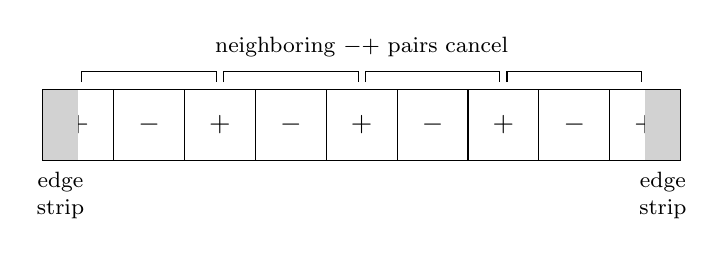
\begin{tikzpicture}[x=0.9cm, y=0.9cm]
  \foreach \i in {0,...,8} {
    \draw (\i,0) rectangle (\i+1,1);
    \ifodd\i \node at (\i+0.5,0.5) {$-$}; \else \node at (\i+0.5,0.5) {$+$}; \fi
  }
  \fill[gray!35] (0,0) rectangle (0.5,1);
  \fill[gray!35] (8.5,0) rectangle (9,1);
  \draw (0,0) rectangle (9,1);
  \foreach \i in {0.5,2.5,4.5,6.5} {
    \draw (\i+0.05,1.1) -- (\i+0.05,1.25) -- (\i+1.95,1.25) -- (\i+1.95,1.1);
  }
  \node[font=\footnotesize] at (4.5,1.6) {neighboring $-{}+$ pairs cancel};
  \node[font=\footnotesize, align=center] at (0.25,-0.5) {edge\\strip};
  \node[font=\footnotesize, align=center] at (8.75,-0.5) {edge\\strip};
\end{tikzpicture}
\caption{One row of half-wavelength regions of a subsonic mode. Pairs cancel; only
the unpaired strips at the edges (gray, and in 2D the corners) are left to radiate.}
\label{fig:edge_radiation}
\end{figure}

% ---------------------------------------------------------------------
\section{What the resonators change}

\subsection{They add small-$k$ states at $1270\,\mathrm{Hz}$}
At $1260\,\mathrm{Hz}$ the bare plate has no choice: every free motion has
$k = k_b = 31.8\,\mathrm{rad/m}$. The flat resonator branch
(Chapter~\ref{ch:local_resonance}) provides modes at about $1270\,\mathrm{Hz}$
for \emph{every} $\mathbf{k}$ in the Brillouin zone, including small $|\mathbf{k}|$
inside the radiation cone (Figure~\ref{fig:radiation_dispersion}). The resonators
do not smooth out the bare mode; they create a kind of mode that the bare plate
cannot have at this frequency.

\subsection{What a flat-branch mode looks like}
By Bloch's theorem (Chapter~\ref{ch:bloch}) a mode on the flat branch is
\begin{equation}
  w(\mathbf{x}) = e^{i\mathbf{k}\cdot\mathbf{x}}\; p(\mathbf{x}),
  \qquad p \text{ cell-periodic},
\end{equation}
a slowly varying envelope $e^{i\mathbf{k}\cdot\mathbf{x}}$ times the same cell
pattern $p$ in every cell.

\paragraph{The cell pattern near $\Gamma$.}
In the in-phase mode the resonator mass bounces on its spring and the plate cell
recoils. With the resonator amplitude $u$ and the mean plate displacement
$\bar w$ of the cell, momentum balance per cell (no external force) gives
\begin{equation}
  m\,u + \rho h A\, \bar w = 0
  \quad\Longrightarrow\quad
  \bar w = -\mu\, u = -0.25\,u .
\end{equation}
The whole cell moves opposite to the resonator with a quarter of its amplitude. On
top of that sits a local dimple under the attachment point, where the spring force
bends the plate (Figure~\ref{fig:cell_pattern}). The dimple is what lowers the
frequency from $f_r\sqrt{1+\mu} = 1342\,\mathrm{Hz}$ (rigid cell) to the FE value
of $1273\,\mathrm{Hz}$ (Chapter~\ref{ch:gap_position}).

\begin{figure}[htbp]
\centering
\begin{tikzpicture}[x=1cm, y=1cm, >={Stealth}]
  % undeformed plate (reference)
  \draw[gray, dashed] (0,0) -- (5,0);
  \node[gray, font=\footnotesize, left] at (0,0) {rest};
  % deformed plate: shifted down by 0.25 with a dimple at x = 2.5
  \draw[thick] plot[domain=0:5, samples=150] (\x, {-0.35 - 0.25*exp(-((\x-2.5)^2)/0.15)});
  % spring
  \draw (2.5,-0.6) -- (2.5,-0.45) -- (2.35,-0.35) -- (2.65,-0.15) -- (2.35,0.05)
        -- (2.65,0.25) -- (2.35,0.45) -- (2.5,0.55) -- (2.5,0.7);
  % mass
  \draw[fill=gray!30] (2.1,0.7) rectangle (2.9,1.2);
  \node[font=\footnotesize] at (2.5,0.95) {$m$};
  \draw[->, thick] (3.2,0.95) -- (3.2,1.55) node[right, font=\footnotesize] {$u$};
  \draw[->, thick] (4.4,-0.05) -- (4.4,-0.35) node[right, font=\footnotesize] {$\bar w = -\mu u$};
  \node[font=\footnotesize] at (1.0,-0.85) {one cell ($10\,\mathrm{cm}$)};
  \node[font=\footnotesize] at (3.6,-0.85) {dimple};
\end{tikzpicture}
\caption{Cell pattern of the in-phase mode near $\Gamma$ (exaggerated): the cell
moves down as a whole while the resonator moves up, with a local dimple at the
attachment point.}
\label{fig:cell_pattern}
\end{figure}

\paragraph{The finite plate.}
The 40 modes of the finite plate between $1246$ and $1282\,\mathrm{Hz}$ are
66--78\,\% resonator motion. Each repeats the cell pattern under a smooth envelope
that varies over the whole plate, like the low-order modes of a $10 \times 10$ grid
of masses. Split the plate motion into two parts (Figure~\ref{fig:smooth_ripple}):
\begin{itemize}
  \item the \textbf{smooth part}: cell means $\bar w$ times the envelope;
  \item the \textbf{ripple}: the dimples, repeated in every cell.
\end{itemize}

\begin{figure}[htbp]
\centering
\begin{tikzpicture}[x=1cm, y=1cm, >={Stealth}]
  % resonator amplitudes following the envelope sin(pi x / 10), 10 cells over 10 units
  \begin{scope}[yshift=3.6cm]
    \foreach \i in {0,...,9} {
      \pgfmathsetmacro{\amp}{0.7*sin((\i+0.5)*18)}
      \draw[->, thick] (\i+0.5,0) -- (\i+0.5,\amp);
    }
    \draw[gray] (0,0) -- (10,0);
    \node[font=\footnotesize, left] at (0,0.3) {resonators};
  \end{scope}
  % smooth part
  \begin{scope}[yshift=2.2cm]
    \draw[gray, dashed] (0,0) -- (10,0);
    \draw[thick] plot[domain=0:10, samples=100] (\x, {-0.5*sin(\x*18)});
    \node[font=\footnotesize, left, align=right] at (0,0) {smooth part\\ $k \approx \pi/L$};
  \end{scope}
  % ripple
  \begin{scope}[yshift=1.0cm]
    \draw[gray, dashed] (0,0) -- (10,0);
    \draw[thick] plot[domain=0:10, samples=400] (\x, {-0.2*sin(\x*18)*exp(-((\x-floor(\x)-0.5)^2)/0.02)});
    \node[font=\footnotesize, left, align=right] at (0,0) {ripple\\ $k \ge 2\pi/a$};
  \end{scope}
  % total
  \begin{scope}[yshift=-0.4cm]
    \draw[gray, dashed] (0,0) -- (10,0);
    \draw[thick] plot[domain=0:10, samples=400] (\x, {-0.5*sin(\x*18) - 0.2*sin(\x*18)*exp(-((\x-floor(\x)-0.5)^2)/0.02)});
    \node[font=\footnotesize, left] at (0,0) {plate};
  \end{scope}
  \draw[|<->|] (0,-1.3) -- (10,-1.3) node[midway, below, font=\footnotesize] {$L = 1\,\mathrm{m}$, 10 cells};
\end{tikzpicture}
\caption{A low-order cluster mode (side view, schematic). Top: resonator
amplitudes follow a smooth envelope. Below: the plate motion is a smooth part
(cell means, opposite to the resonators) plus a ripple of dimples, one per cell.}
\label{fig:smooth_ripple}
\end{figure}

\subsection{Which part radiates}
\begin{center}
\begin{tabular}{|l|p{0.28\textwidth}|p{0.18\textwidth}|p{0.27\textwidth}|}
\hline
Part & Wavenumbers & vs.\ $k_\mathrm{air} = 23.1\,\mathrm{rad/m}$ & Radiates? \\
\hline
smooth part & envelope: $m\pi/L = 3.1, 6.3, 9.4, \dots\,\mathrm{rad/m}$ & inside the cone for low orders & yes: $+$ and $-$ regions tens of cm apart \\
ripple & $\ge 2\pi/a = 62.8\,\mathrm{rad/m}$ & far outside & no: decay length $1/\sqrt{62.8^2 - 23.1^2}\,\mathrm{m} = 1.7\,\mathrm{cm}$ \\
\hline
\end{tabular}
\end{center}
In the extreme case of a uniform envelope ($\mathbf{k} = 0$), all cell means move in
phase and the plate acts as a piston. A rough estimate (not computed): envelope
orders up to $m \approx 7$ satisfy $m\pi/L < 23.1\,\mathrm{rad/m}$ on the
$1\,\mathrm{m}$ plate, which fits the observation that most, but not all, cluster
modes radiate strongly.

\paragraph{Why the plate simply follows the resonators.}
For a force pattern with wavenumber $k$ the plate responds (Kirchhoff, undamped) with
\begin{equation}
  \hat w(k) = \frac{\hat F(k)}{D k^4 - \rho h\,\omega^2}
  \;\overset{k \ll k_b}{\approx}\; -\frac{\hat F(k)}{\rho h\,\omega^2} .
\end{equation}
At small $k$ the bending stiffness $D k^4$ is negligible; the plate acts like a mass
and moves with whatever smooth pattern the resonators impose. The plate goes where
the resonators push it, and they push smoothly.

\subsection{The numbers}
From the modal analysis of the finite plate (open check (b),
\texttt{check\_finite\_plate\_modes.py}):
\begin{center}
\begin{tabular}{|l|l|}
\hline
Modes & Radiation efficiency $\sigma$ \\
\hline
bare plate, near $1260\,\mathrm{Hz}$ & $0.003$--$0.014$ \\
cluster $1246$--$1282\,\mathrm{Hz}$, $2\times 2$ shear rule & $0.35$--$0.90$ \\
cluster, full $3\times 3$ shear rule & $0.54$--$0.80$ \\
\hline
\end{tabular}
\end{center}
Per unit velocity the cluster modes radiate about $20\,\mathrm{dB}$ more than the bare
modes. In Eq.~\eqref{eq:il_split} the efficiency term is then about
$10\log_{10}(0.01/0.5) \approx -17\,\mathrm{dB}$, which the velocity term cannot
compensate: the IL dips to about $-14\,\mathrm{dB}$. (Rough: in the forced response
several modes overlap, so the modal $\sigma$ values only bracket the effective one.)
With the full $3\times 3$ shear rule, now used throughout, the dip is
$-13.9\,\mathrm{dB}$ at $1267\,\mathrm{Hz}$.

\paragraph{Inside a gap: the $600\,\mathrm{Hz}$ tuning.} The same mechanism can reach into
a gap. With $f_r = 600\,\mathrm{Hz}$ ($\tau = 0.5$, Bloch gap $578$--$662\,\mathrm{Hz}$) the
IL turns negative from $633\,\mathrm{Hz}$ on, about $65\,\%$ into the gap. Averaged over
$628$--$662\,\mathrm{Hz}$: IL $-7.4\,\mathrm{dB}$ = velocity term $+7.8\,\mathrm{dB}$ +
efficiency term $-15.2\,\mathrm{dB}$. The plate does move less, as the gap requires, but the
remaining motion radiates far better. At this tuning the upper gap edge \emph{is} the
resonator band at $\Gamma$ (small $k$, supersonic), and the bare plate, four times below
$f_c$, radiates very poorly. At $1200\,\mathrm{Hz}$ the upper edge is the sin pattern at
$X$, which is subsonic ($31.4$ against $21.9\,\mathrm{rad/m}$), and the efficiency term
inside the gap stays near $-3\,\mathrm{dB}$.

% ---------------------------------------------------------------------
\section{Summary}
\begin{enumerate}
  \item Below $f_c \approx 2.4\,\mathrm{kHz}$ free bending waves are subsonic
        ($k_b > k_\mathrm{air}$); the air short-circuits between neighboring crests
        and troughs, and only edges and corners radiate ($\sigma \sim 0.01$).
  \item The flat resonator branch provides modes at about $1270\,\mathrm{Hz}$ for all
        $\mathbf{k}$, including small $\mathbf{k}$ inside the radiation cone.
  \item In these modes the plate moves as cell means (opposite to the resonators,
        $\bar w = -\mu u$) under a smooth envelope, plus a ripple of dimples. The
        smooth part is supersonic and radiates ($\sigma \sim 0.5$); the ripple does not.
  \item The plate does not move more, it moves in a shape the air cannot short-circuit:
        the efficiency term of the IL is about $-17\,\mathrm{dB}$, giving the
        $-14\,\mathrm{dB}$ dip.
\end{enumerate}

% ---------------------------------------------------------------------
\section{Check questions with answers}

\paragraph{Question 1.} \emph{Would the bare plate radiate better at
$2000\,\mathrm{Hz}$ than at $1260\,\mathrm{Hz}$? Use the wavenumbers.}

\emph{Answer.} Yes. $k_b \propto \sqrt{f}$: $k_b(2000) = 31.8\sqrt{2000/1260} =
40.1\,\mathrm{rad/m}$, while $k_\mathrm{air}(2000) = 2\pi\cdot 2000/343 =
36.6\,\mathrm{rad/m}$. Still subsonic, but much closer to coincidence: the decay
length grows from $4.6\,\mathrm{cm}$ to $1/\sqrt{40.1^2 - 36.6^2}\,\mathrm{m} \approx
6.1\,\mathrm{cm}$, and crest and trough are $7.8\,\mathrm{cm}$ apart against
$8.6\,\mathrm{cm}$ covered by sound in half a period. The short circuit becomes
incomplete; $\sigma$ rises towards its maximum near $f_c$.

\paragraph{Question 2.} \emph{The resonators push hardest right at the attachment
points, where the dimples are. Why does that motion not radiate?}

\emph{Answer.} The dimples repeat with the lattice period, so their wavenumbers are at
least $2\pi/a = 62.8\,\mathrm{rad/m}$, almost three times $k_\mathrm{air}$. Their
pressure decays with a length of $1.7\,\mathrm{cm}$: each dimple is short-circuited by
the surrounding plate, which moves the other way. Only the cell means, collected under
a smooth envelope, reach the far field.

\paragraph{Question 3.} \emph{Resonators tuned to $3\,\mathrm{kHz}$, above $f_c$: would
the same IL dip appear at their flat branch?}

\emph{Answer (expectation, not computed).} Much weaker. Above $f_c$ the bare plate's
free waves are already supersonic and radiate with $\sigma \approx 1$. The flat branch
cannot raise $\sigma$ much further, so the efficiency term of
Eq.~\eqref{eq:il_split} is small, and the IL is governed by the velocity term. The dip
is a below-coincidence effect.
